\documentclass[times,review,10pt]{elsarticle}
%% Compiled with pdfLaTeX using the journal's exact required class options
%% (times, review, 10pt). The manuscript text is plain ASCII (the one
%% Vietnamese place name with diacritics, "Cu Chi", was written without
%% diacritics for this reason), so no extra Unicode/font packages are needed.
\usepackage[utf8]{inputenc}
\usepackage[T1]{fontenc}

\usepackage{graphicx}
\usepackage{booktabs}
\usepackage{array}
\usepackage{caption}
\usepackage{amsmath}
\usepackage[hyphens]{url}
\usepackage{hyperref}
\hypersetup{colorlinks=true, linkcolor=blue, citecolor=blue, urlcolor=blue, breaklinks=true}
\setlength{\emergencystretch}{2em}

\setlength{\tabcolsep}{4pt}
\renewcommand{\_}{\textunderscore\allowbreak}

\usepackage{float}
\usepackage{placeins}
\renewcommand{\topfraction}{0.95}
\renewcommand{\bottomfraction}{0.9}
\renewcommand{\textfraction}{0.05}
\setcounter{topnumber}{4}
\setcounter{bottomnumber}{4}
\setcounter{totalnumber}{8}

\journal{Pattern Recognition}

\begin{document}

\begin{frontmatter}

\title{ChiliEdgeNet: A Lightweight CNN-Transformer Hybrid Toward On-Device Chili Pepper Disease Recognition}

\author[a,b]{Minh Hai To}
\author[a,b,c]{Tien Do}
\author[c]{Bao The Phung\corref{cor1}}
\cortext[cor1]{Corresponding author.}
\ead{baopt@huit.edu.vn}

\affiliation[a]{organization={Faculty of Information Science and Engineering, University of Information Technology},
            city={Ho Chi Minh City},
            postcode={700000},
            country={Vietnam}}
\affiliation[b]{organization={Vietnam National University Ho Chi Minh City},
            city={Ho Chi Minh City},
            postcode={700000},
            country={Vietnam}}
\affiliation[c]{organization={Ho Chi Minh City University of Industry and Trade},
            city={Ho Chi Minh City},
            postcode={700000},
            country={Vietnam}}

\begin{abstract}
Plant-disease diagnosis for resource-constrained devices requires models that balance accuracy, efficiency, and robustness. This work proposes ChiliEdgeNet, a lightweight CNN-Transformer hybrid built by truncating MobileNetV2 and integrating a Tiny Transformer block. We also introduce ChiliEdge-DS, a public dataset containing 2,461 chili pepper leaf and fruit images across five classes. ChiliEdgeNet achieves 98.93\% accuracy with 671,173 parameters, approximately 35\% fewer than the base architecture. The model occupies 2.7 MB and reaches 20.24 ms/image inference latency on a server-class CPU. Under synthetic brightness reduction at factor 0.2, the full model outperforms the no-Transformer variant by 3.75 percentage points. On an external 1,463-image Mendeley query set spanning four classes, accuracy improves from 30.96\% to 89.75\% after adaptation using only 42 support images. These results demonstrate strong potential for offline deployment, while direct edge-hardware testing and broader cross-domain validation remain necessary. Further evaluation is needed before suitability for resource-constrained agricultural deployment can be confirmed.
\end{abstract}

\begin{keyword}
chili pepper disease classification \sep lightweight deep learning \sep CNN--Transformer \sep edge AI \sep few-shot domain adaptation \sep explainable AI
\end{keyword}

\end{frontmatter}

\FloatBarrier

\section{Introduction}\label{introduction}

Early detection of plant disease from images can support monitoring and treatment. However, deployment at the point of image capture requires a model with low computational cost, offline operation, and sufficiently high accuracy \cite{joseph2024,maurya2024,duhan2025}, requirements that matter most for resource-constrained devices. Chili pepper disease detection specifically has also been explored recently, from a disease-and-pest detection framework \cite{kanaparthi2026} to a precision-agriculture deployment study in another growing region \cite{odounfa2025}, though neither targets the offline, resource-constrained setting addressed here.

Lightweight CNNs offer an advantage in parameter count and local spatial inductive bias; a sufficiently deep network can still reach a large receptive field, but it does not directly model pairwise interactions between every position the way self-attention does. Vision Transformers support exploiting global relations, but standard configurations typically carry higher computational cost \cite{gole2023,li2023}. Hybrid CNN-Transformer architectures can therefore reconcile the two properties.

Within the body of work surveyed in Section 2, results are reported on different datasets and protocols, so they do not yet form a shared comparison that simultaneously analyzes each component's contribution, response to synthetic degradation, and background domain gap. The gap considered here is not the absolute absence of each individual analysis, but the absence of a protocol that combines these evaluation axes on the same data split and training procedure. In particular, high accuracy on a controlled-background dataset does not guarantee performance on natural-background images. XAI is used to probe prediction behaviour, while a general-purpose multimodal model provides a reference comparison.

Building on the RTR\_Lite\_MobileNet architecture \cite{duhan2025}, based on MobileNetV2 \cite{sandler2018}, this work proposes ChiliEdgeNet, a CNN-Transformer hybrid under 700 thousand parameters.

The main contributions of this work are summarized as follows:

\begin{enumerate}
\item \textbf{Lightweight CNN--Transformer architecture.} We propose ChiliEdgeNet, a compact hybrid architecture that achieves 98.93\% accuracy with 671,173 parameters, approximately 35\% fewer than the base architecture under the same seed-42 protocol. The model occupies 2.7 MB and achieves an inference latency of 20.24 ms/image on a Kaggle virtual-machine CPU.

\item \textbf{ChiliEdge-DS dataset.} We introduce ChiliEdge-DS, a dataset containing 2,461 chili pepper leaf and fruit images across five classes, collected in southern Vietnam under a controlled white-background setting. The dataset is divided into fixed training, validation, and test sets and publicly released on \href{https://drive.google.com/drive/folders/1DesS0c5xT6J72tIv8AMZLwC8ANFUk2PC?usp=drive_link}{ChiliEdge-DS}.

\item \textbf{Controlled robustness and cross-dataset evaluation.} We conduct retrain-from-scratch architectural ablations and synthetic degradation experiments under a fixed seed-42 protocol. We further evaluate cross-dataset transfer on a clean query set of 1,463 images across four mapped classes from Mendeley Data. Accuracy improves from 30.96\% at the original checkpoint to 89.75\% after adaptation with only 42 support images. The support and query sets have zero SHA-256 intersection, and paired analysis records 870 incorrect-to-correct transitions and only 10 regressions.

\item \textbf{Model interpretation and multimodal reference comparison.} We employ three complementary XAI methods for qualitative analysis of ChiliEdgeNet's prediction behaviour. In addition, a general-purpose multimodal model is evaluated zero-shot on all 373 test images as a reference comparison rather than as a peer baseline.

\item \textbf{Laptop-camera integration and deployment-oriented evaluation.} We integrate ChiliEdgeNet into a laptop-camera application and evaluate 62 batch-size-1 predictions on an Intel Core i7-13650HX CPU. The median preprocessing-and-inference latency is 29.70 ms. This measurement excludes frame capture, ROI cropping, pre-ROI format conversion, UI rendering, and file writing, and therefore should not be interpreted as camera FPS or full-pipeline latency.

\end{enumerate}


\FloatBarrier

\section{Related Work}\label{related-work}

\subsection{Baseline Selection Criteria}\label{baseline-selection-criteria}

\textbf{Selection criteria for the baseline pool.} Table 4 comprises 17 baselines from 15 studies, selected on the basis of peer-reviewed work published 2023--2026 on image-based plant-disease classification; a clear architectural focus on deployability (lightweight CNN / ViT / hybrid) or a broad CNN-vs-ViT comparative study; architectural detail sufficient (layer configuration, embedding widths, head counts) to reproduce or adapt for the target task without contacting the authors; and coverage of the four directions below rather than only the strongest family.

Studies were excluded when they targeted detection/segmentation rather than classification, or when no corresponding classification output could be constructed. The baseline pool therefore represents the deployment-oriented literature of the last three years, not an exhaustive survey; the models were reimplemented and evaluated by us under a common protocol described in Section 4.1, so Table 4 does not use the figures originally published by the authors.

Studies that perform only detection or segmentation with no image-level classification output were excluded from the baseline pool. Multitask models are kept if the original architecture has an explicit classification branch that can be adapted to the target task; Table 2 details the specific adaptation applied to the one such case in the pool, PDLC-ViT \cite{hemalatha2024}.

\subsection{Related Architectural Directions}\label{related-architectural-directions}

\textbf{Lightweight CNNs} keep parameters low through efficient attention or compact blocks: RTR\_Lite\_MobileNetV2 \cite{duhan2025}, our base architecture, adds triplet attention \cite{misra2021} and a spatial-attention residual block to MobileNetV2 \cite{sandler2018}; ULEN \cite{wang2023} pushes ultra-lightweight design down to 28 thousand parameters; MRW-CNN \cite{joseph2024} and Lite-MDC \cite{bhagat2024} target real-time field deployment; and CustomMNetV3L \cite{rahaman2026} adapts MobileNetV3-Large. \textbf{Vision Transformers} directly exploit relations between tokens, unlike deep CNNs, which can extend the receptive field to aggregate broad context but do not directly model pairwise interactions between every position; ViTs typically carry higher cost, as in ViT \cite{ali2025}, TrIncNet \cite{gole2023} with a Trans-Inception block, PMVT \cite{li2023} for mobile deployment, PDLC-ViT \cite{hemalatha2024} for multitask localization plus classification, and a multi-kernel inception-enhanced ViT \cite{hassan2025} for improved feature diversity. \textbf{Hybrid CNN-Transformer architectures} closest to this line of work include GrapeLeafNet \cite{karthik2024}, MaizeFormerX \cite{rahman2026}, and LDI-NET \cite{yangB2024}, typically at 3--9 million parameters; more recent designs include ConvTransNet-S for complex field backgrounds \cite{jia2025}, a lightweight CNN-ViT for maize \cite{mehdipour2026}, and a lightweight CNN-Transformer with built-in explainability for medicinal-leaf disease \cite{ahmmed2026}. \textbf{Broad comparative studies} include Mishra et al. \cite{mishra2026}, Sujatha et al. \cite{sujatha2025}, and the lightweight IoT meta-ensemble of Maurya et al. \cite{maurya2024}.

These works use different datasets, splits, and training protocols, so they do not yet form a single shared comparison across architectural contribution, degradation robustness, and domain gap.

\FloatBarrier

\section{Proposed Method}\label{proposed-method}

\subsection{Dataset}\label{dataset}

ChiliEdge-DS comprises 2,461 chili pepper leaf and fruit images across five classes: \emph{anthracnose}, \emph{healthy}, \emph{leaf\_curl}, \emph{leaf\_spot}, and \emph{yellow\_leaf}. The images were collected by the author in the Cu Chi area, Ho Chi Minh City, Vietnam. The data was split once, at an approximate 65:20:15 ratio, into \emph{train}, \emph{val}, and \emph{test} sets of 1,597, 491, and 373 images respectively (Table 1). This fixed split is kept unchanged throughout all main experiments.

Images were taken against a white background using a smartphone camera; the device model was not recorded. Images have a native resolution of approximately 12,000 × 9,000 pixels, saved at 300 × 300 pixels, and resized to 224 × 224 for model input. The dataset is publicly released on Kaggle \cite{to2026c}.

Labels were assigned manually by the author based on visual presentation: \emph{anthracnose} shows dark, necrotic lesions on the leaf or fruit surface; \emph{healthy} shows no clearly observable symptoms; \emph{leaf\_curl} shows leaf curling or twisting; \emph{leaf\_spot} shows discrete lesion spots on the leaf surface; and \emph{yellow\_leaf} shows predominant leaf yellowing. These are phenotype-based labels from visual observation, not pathogen identification confirmed by laboratory testing.

ChiliEdge-DS is hosted on a private Google Drive repository and can be made available upon reasonable request \cite{to2026c}.

The ratio between the largest and smallest class is 1.29, so no class weighting was applied. Macro-F1 is reported alongside accuracy so that each class contributes equally to the aggregate result. The white background is a controlled acquisition condition; the gap with other-source images and natural backgrounds is examined in Section 4.5 and discussed in Section 6.

\begin{table}[H]
\centering
\caption*{\textbf{Table 1.} Per-class distribution of ChiliEdge-DS across the fixed split.}
\label{tab:1}
\footnotesize
\renewcommand{\arraystretch}{1.15}
\begin{tabular}{lllll}
\toprule
\textbf{Class} & \textbf{Train} & \textbf{Val} & \textbf{Test} & \textbf{Total} \\
\midrule
anthracnose & 264 & 81 & 62 & 407 \\
healthy & 334 & 102 & 78 & 514 \\
leaf\_curl & 328 & 104 & 82 & 514 \\
leaf\_spot & 326 & 101 & 76 & 503 \\
yellow\_leaf & 345 & 103 & 75 & 523 \\
\textbf{Total} & \textbf{1,597} & \textbf{491} & \textbf{373} & \textbf{2,461} \\
\bottomrule
\end{tabular}
\end{table}

\subsection{Architecture: ChiliEdgeNet}\label{architecture-chiliedgenet}

CNNs exploit local features well but remain limited in directly modelling relations between distant regions. ChiliEdgeNet therefore combines a truncated MobileNetV2 with a Tiny Transformer block (Fig. 1). Relative to the base architecture \cite{duhan2025}, it also omits Triplet Attention \cite{misra2021} and a \emph{RES\_Block} combining ECA with SE; Section 4.3 reports the ablation evidence behind this choice.

\subsubsection{Backbone Cut Point}\label{backbone-cut-point}

ChiliEdgeNet uses MobileNetV2 pretrained on ImageNet and keeps the layers from \emph{features{[}0{]}} to \emph{features{[}13{]}}. With a 224 × 224 input, the backbone produces a feature map of size 96 × 14 × 14, corresponding to 196 spatial positions.

The backbone is cut before \emph{features{[}14{]}}, because this layer reduces the feature map to 7 × 7 and the token count from 196 to 49. The cut point \emph{cut = 14} was chosen through a preliminary sweep and also gives the Attention Rollout map four times as many spatial positions as a 7 × 7 grid.

\subsubsection{Feature Processing Path}\label{feature-processing-path}

The image is processed through the following pipeline: MobileNetV2 \emph{features{[}0:14{]}}; a Conv 1 × 1 layer mapping 96 to 128 channels; BatchNorm, GELU, and dropout 0.1; flattening the feature map into 196 image tokens, each with 128 dimensions; the Tiny Transformer block; RMSNorm and mean pooling over the token dimension; and, finally, dropout 0.2 followed by a linear layer predicting five classes.

\subsubsection{Tiny Transformer Block}\label{tiny-transformer-block}

ChiliEdgeNet is a purely vision-based model, using no text encoder, tokenizer, or pretrained language weights. The Tiny Transformer uses a pre-norm structure consisting of RMSNorm followed by GQA combined with 2D-RoPE and a residual connection, followed in turn by RMSNorm, an MLP with GELU, and a second residual connection.

The model uses embedding dimension 128, four query heads, two key/value heads, an MLP ratio of 2, and dropout of 0.1.

Three parameter-efficient techniques are used. \textbf{2D-RoPE}: rotary position embedding rotates each pair of query/key components by a position-dependent angle \cite{su2024}, using an axial variant for the image grid that rotates one half of each head by the row coordinate and the other half by the column coordinate, following the RoPE-Axial extension for Vision Transformers of Heo et al. \cite{heo2025}; this replaces a learned positional-embedding table, saving 25,088 parameters. \textbf{GQA}: grouped-query attention lets four query heads share two key/value heads \cite{ainslie2023}, saving 16,384 parameters compared with four-head multi-head attention; the benefit quantified here is a reduction in projection parameters and is not extrapolated into a claim about inference-speed gains. \textbf{RMSNorm}: this replaces LayerNorm by normalizing with the root-mean-square rather than subtracting the mean, with no shift bias \cite{zhang2019}, saving a total of 384 parameters; this is an exact structural difference, and RMSNorm's effect on accuracy still must be confirmed by ablation rather than inferred directly from the parameter count.

Together these three techniques save 41,856 parameters, roughly 6.2\% of ChiliEdgeNet's parameter count. The model has 671,173 parameters, about 35.0\% fewer than the base architecture \cite{duhan2025}, which has 1,032,568 parameters.

\begin{figure*}[!tb]
\centering
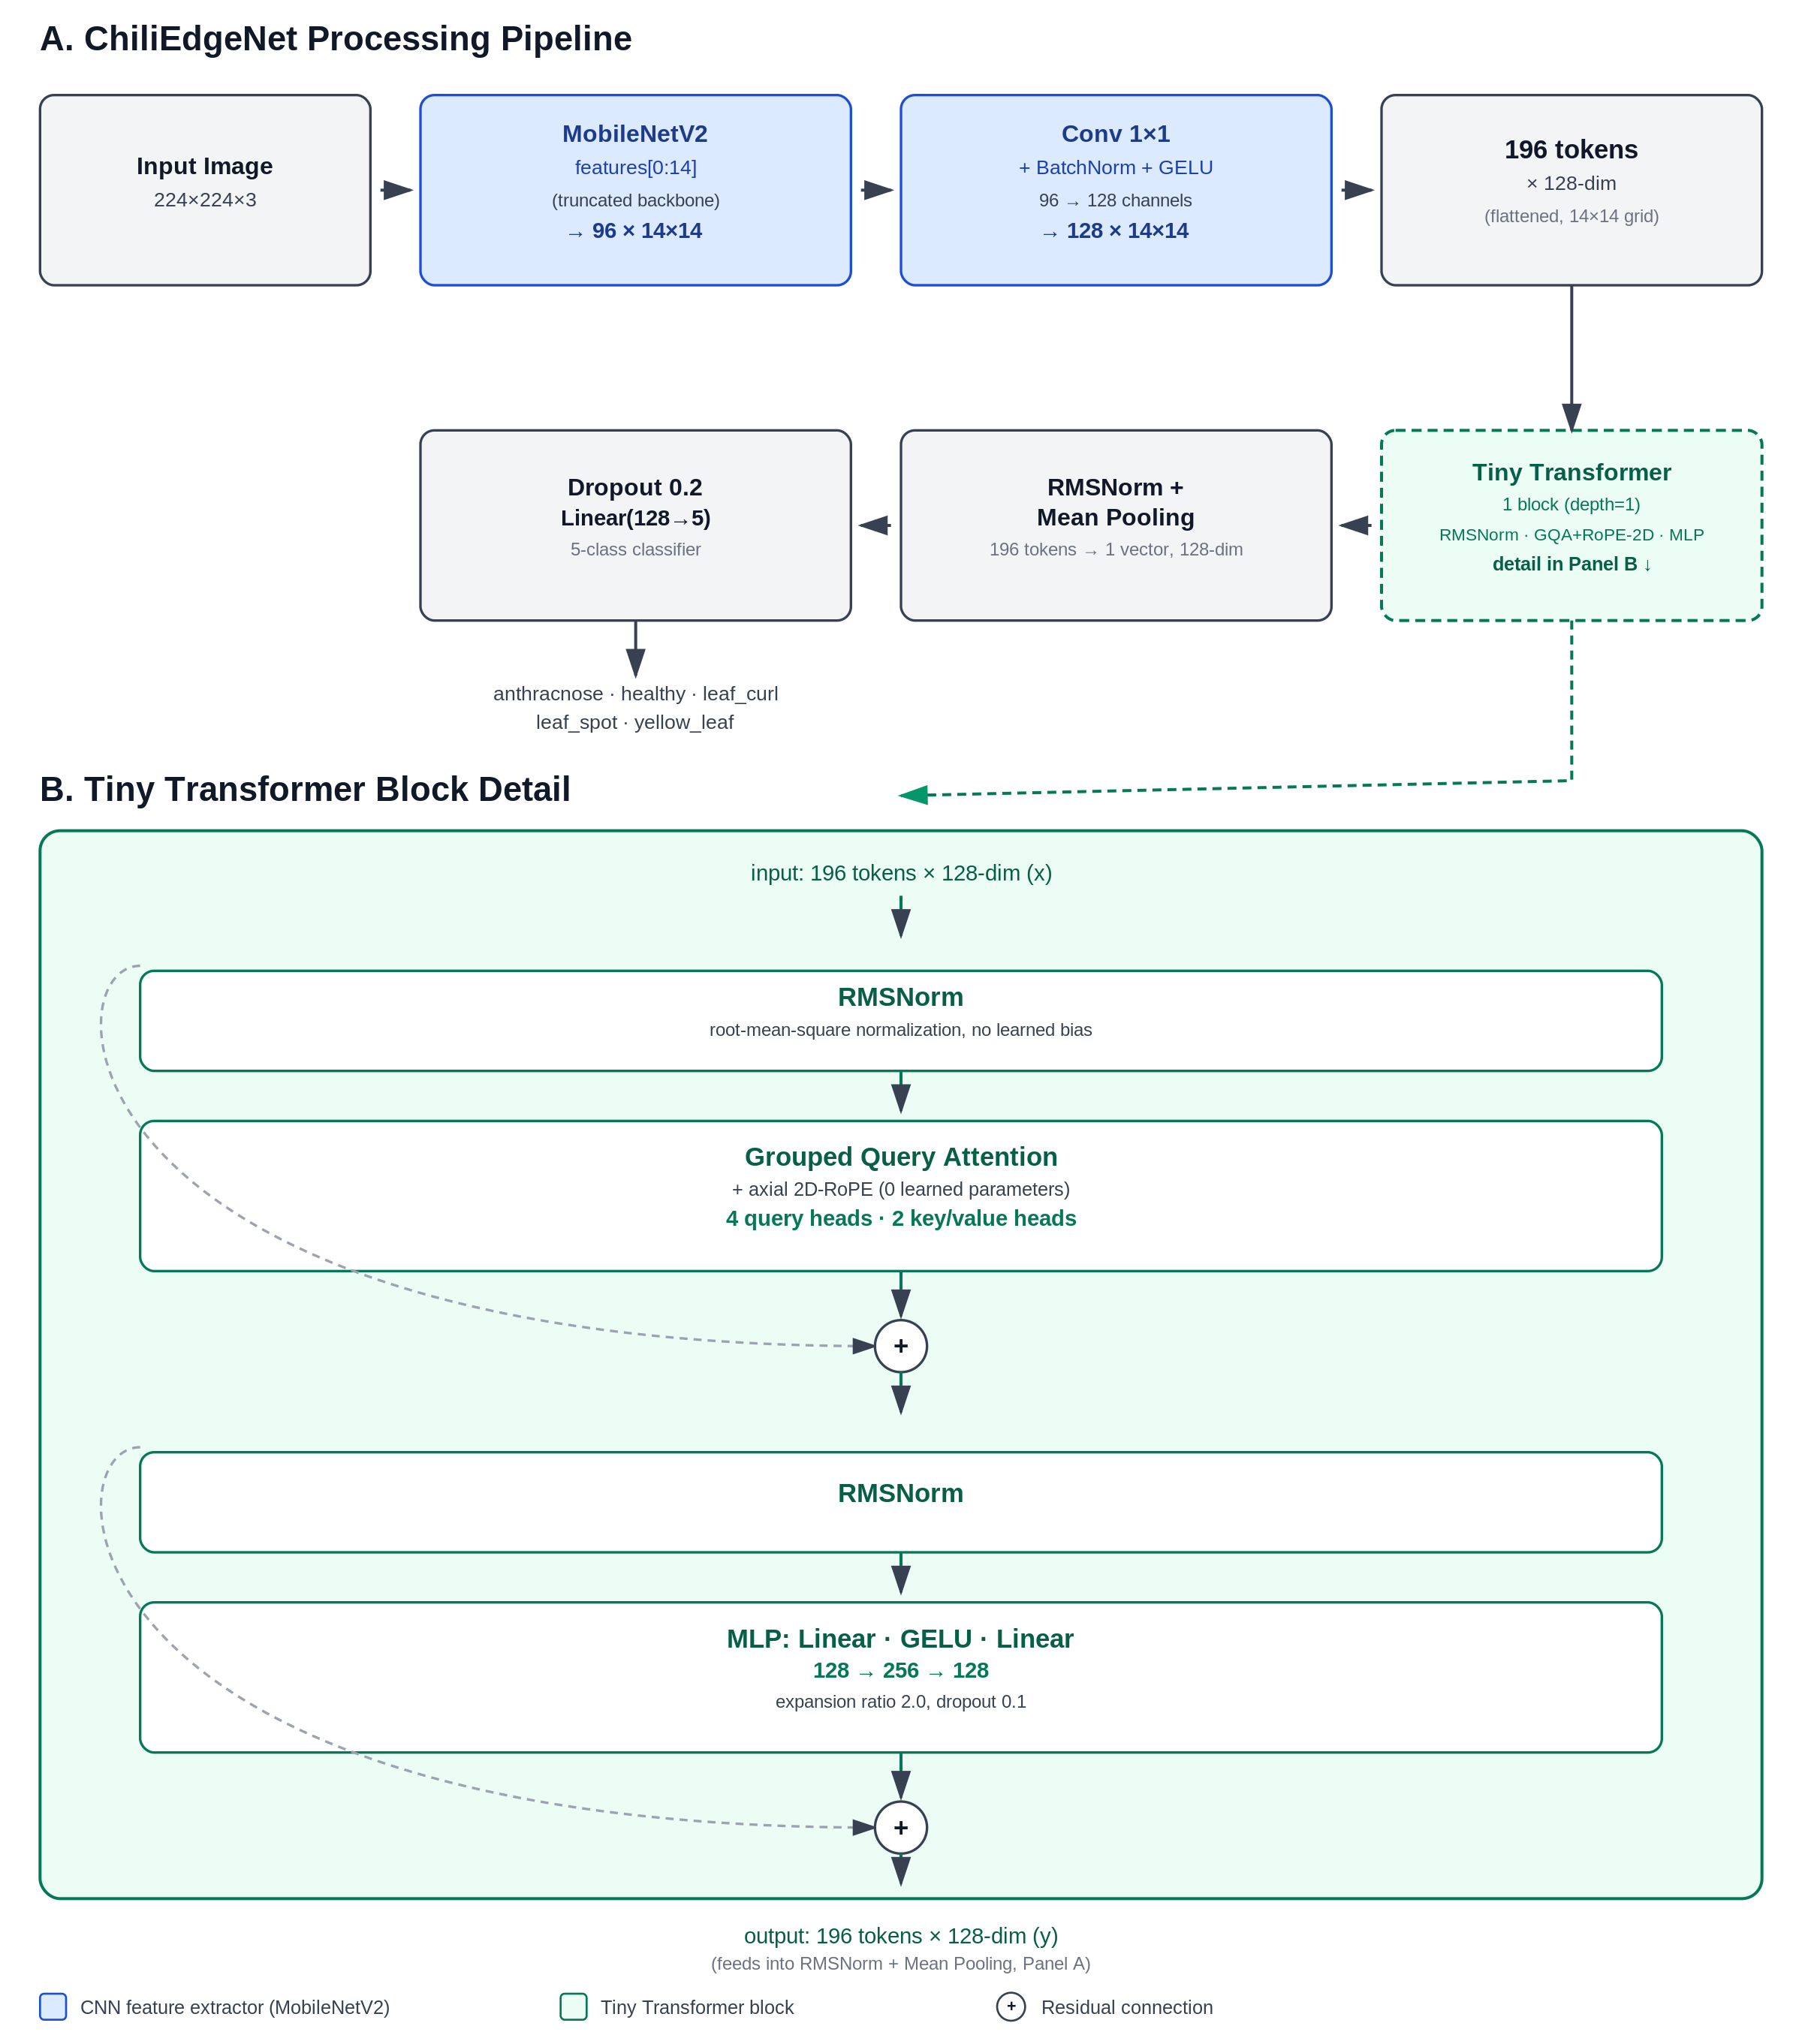
\includegraphics[width=0.85\linewidth,height=0.42\textheight,keepaspectratio]{figs/fig1_new.png}
\caption*{\textbf{Fig.\ 1.} ChiliEdgeNet architecture. Panel A: overall pipeline from the 224x224x3 input through the truncated MobileNetV2 backbone (features{[}0:14{]}), a 1x1 convolution reducing channels, 196 tokens, the Tiny Transformer block, mean pooling and the classifier, with tensor shapes at each step. Panel B: detail of one Tiny Transformer block, showing RMSNorm, Grouped Query Attention with axial 2D-RoPE (4 query heads, 2 key/value heads) with a residual connection, and a GELU MLP (expansion ratio 2.0) with a residual connection.}
\label{fig:1}
\end{figure*}

\subsection{Evaluation Metrics}\label{evaluation-metrics}

This work reports top-1 accuracy, macro-F1, and total parameter count. Every test-set accuracy value carries a 95\% Wilson confidence interval at $N = 373$. Accuracy is the proportion of correctly predicted images out of $N$. For each class, precision and recall are computed from true positives (TP), false positives (FP), and false negatives (FN):

\begin{equation}
\text{Precision} = \frac{TP}{TP+FP}, \qquad \text{Recall} = \frac{TP}{TP+FN}
\end{equation}

\begin{equation}
F1 = \frac{2 \times \text{Precision} \times \text{Recall}}{\text{Precision}+\text{Recall}}
\end{equation}

Macro-F1 is the unweighted average of the per-class F1 score across the five classes, so that each class contributes equally regardless of its size.

\FloatBarrier

\section{Experiments and Results}\label{experiments-and-results}

\subsection{Setup}\label{setup}

Experiments were run on Kaggle with an NVIDIA Tesla T4 GPU; the reproduction code uses PyTorch or TensorFlow depending on the architecture. Each baseline is evaluated under two scenarios: a \textbf{baseline} scenario with no data augmentation applied, and an \textbf{augmented} scenario with the data-augmentation techniques in Table 3 applied.

The \emph{val} and \emph{test} sets are never augmented. For epoch-trained models, the checkpoint with the best validation criterion for each configuration is reloaded before test evaluation.

\textbf{Common evaluation framework.} Seventeen baselines use the same ChiliEdge-DS dataset, the same fixed \emph{train}/\emph{val}/\emph{test} split, seed 42, and the metrics accuracy, macro-F1, and parameter count. Both scenarios are evaluated on the same non-augmented test set. Architecture-dependent settings such as input size, batch size, epoch count, optimizer, and augmentation intensity follow each model's own reproduction design. The comparison is therefore controlled for data, split, and metric, but does not use a fully uniform training recipe across every architecture. Two cases where test results influenced selection---RTR\_Lite\_MobileNet \cite{duhan2025} as the primary baseline and InceptionV3 + SVM as the representative for Sujatha et al. \cite{sujatha2025}---are disclosed in Section 4.2 and interpreted only as exploratory analysis.

The common 17-baseline evaluation framework is limited to in-domain results on the ChiliEdge-DS test set: accuracy, macro-F1, and parameter count. Additional analyses of blur, low light, architectural ablation, XAI, and domain transfer were carried out only for ChiliEdgeNet and its corresponding controlled variants. This work therefore does not present these experiments as a uniform robustness or domain-transfer benchmark for all 17 baselines.

Table 2 summarizes the significant changes applied when adapting each baseline architecture to the five-class task.

\begin{table*}[!tb]
\centering
\caption*{\textbf{Table 2.} Summary of the significant changes applied when adapting each baseline architecture to the five-class task.}
\label{tab:2}
\footnotesize
\renewcommand{\arraystretch}{1.3}
\begin{tabular}{>{\raggedright\arraybackslash}p{0.13\linewidth} >{\raggedright\arraybackslash}p{0.30\linewidth} >{\raggedright\arraybackslash}p{0.50\linewidth}}
\toprule
\textbf{Baseline} & \textbf{Component retained} & \textbf{Component adapted} \\
\midrule
PDLC-ViT (classification-only; \cite{hemalatha2024}) & Co-scale, co-attention, cross-attention, Transformer encoder, and classification head & Segmentation/localization branch removed; converted from multitask to five-class classification using only classification loss; ViT hyperparameters not fully disclosed were set during reproduction. \\
LDI-NET \cite{yangB2024} & Feature Tokenizer and Token Encoder & The multi-label decoder predicting plant type, disease, and severity was replaced with global average pooling and a five-class linear classifier. \\
InceptionV3 + SVM \cite{sujatha2025} & Frozen backbone for feature extraction and SVM for classification & Adapted to ChiliEdge-DS; StandardScaler, PCA retaining 95\% of variance, and the exploratory selection described in Section 4.2 were applied. \\
Meta-Ensemble \cite{maurya2024} & MLP-Mixer, CNN--LSTM branch, and SVM meta-classifier & Output changed to five classes; patch-embedding configuration implemented as set here, since the original description did not provide full detail. \\
\bottomrule
\end{tabular}
\end{table*}

The proposed model and all ablation variants use seed 42 and are re-initialized before each run. In the ablation experiments, configurations therefore differ only in the component removed, added back, or replaced.

\begin{table*}[!tb]
\centering
\caption*{\textbf{Table 3.} Training configuration for ChiliEdgeNet and its ablation variants.}
\label{tab:3}
\small
\renewcommand{\arraystretch}{1.15}
\begin{tabular}{ll}
\toprule
\textbf{Item} & \textbf{Value} \\
\midrule
Input image size & 224 × 224 \\
Baseline transform & Resize, ToTensor, Normalize \\
Augmented transform & 30° rotation, ColorJitter, horizontal flip, affine \\
Epochs & 30 \\
Batch size & 32 \\
Loss function & Cross-entropy, label smoothing 0.05 \\
Learning-rate schedule & 10\% linear warm-up → cosine decay \\
Learning rate (backbone / new blocks) & 1e-4 / 1e-3 \\
Seed & \textbf{42} \\
\bottomrule
\end{tabular}
\end{table*}

\textbf{Run count and statistical testing.} Results for the proposed model and its ablation variants are reported from a single run with seed 42. This work does not report a mean or standard deviation across multiple seeds and does not interpret these results as evidence of stability across initializations. The McNemar test is used to assess the difference between two models on a per-image basis over the same 373-image test set.

For each comparison, the tables report two raw counts, written as b / c, alongside the McNemar $p$-value, where $b$ is the number of images the first model predicts correctly while the second predicts incorrectly, and $c$ is the number of images the first model predicts incorrectly while the second predicts correctly.

McNemar's test checks whether the number of discordant cases in the two directions differs significantly. This test does not substitute for assessing variance across multiple seeds; that limitation is discussed in Section 6.

In this work, McNemar is applied to comparisons between ChiliEdgeNet and its ablation variants on the same 373 test images, corresponding to Tables 6--8, and to the paired comparison of the two checkpoints on the same 1,463 cross-dataset query images in Table 11b. The test is not used to rank all 17 baselines in Table 4.

The base architecture RTR\_Lite\_MobileNet \cite{duhan2025} in Section 4.2 was also reproduced with seed 42. The comparison is therefore seed-matched and follows the same procedure, but each architecture was still run only once.

\textbf{Inference latency measurement.} ChiliEdgeNet's CPU latency is 20.24 ms/image, equivalent to 49.41 images/second, measured on an Intel Xeon 2.00 GHz CPU with 4 logical cores on a Kaggle virtual machine. The measurement setup uses PyTorch FP32, batch size 1, with 10 warm-up iterations and 50 timed iterations. The 49.41 images/second figure is inference throughput converted from a single-image server benchmark, not the FPS of a camera application.

On the same environment, the Tesla T4 GPU reaches 5.46 ms/image at batch size 1 and 0.82 ms/image at batch size 32.

The CPU used is a server-class x86 CPU, not edge hardware. These results therefore reflect only the inference cost in the current experimental environment.

\subsection{Comparison with State-of-the-Art Models}\label{comparison-with-state-of-the-art-models}

At seed 42, ChiliEdgeNet reaches 97.86\% in the baseline scenario and 98.93\% in the augmented scenario. The corresponding macro-F1 values are 0.9790 and 0.9897.

A total of 17 baselines from 15 recent studies were reproduced and evaluated under the same framework, presented in full in Table 4. Because the baselines were each run once and not individually tuned for ChiliEdge-DS, this table reflects results under shared data, split, and metrics, not an absolute ranking between architectures.

RTR\_Lite\_MobileNet \cite{duhan2025} was chosen as the primary baseline because it is the direct base architecture of ChiliEdgeNet and has the highest observed accuracy among the evaluated baselines on the ChiliEdge-DS test set. Since the test result contributed to this baseline selection, the direct comparison with RTR\_Lite\_MobileNet is treated as exploratory analysis on the current split, not an independent test evaluation establishing statistical ranking or a general superiority claim. The parameter reduction remains a structural comparison and does not depend on test-based selection.

For the study by Sujatha et al. \cite{sujatha2025}, ten combinations of two backbones (VGG19 and InceptionV3) with five classifiers (SVM, kNN, Random Forest, AdaBoost, and Decision Tree) were evaluated on the same data split. The InceptionV3 + SVM configuration, which had the highest observed test accuracy, was chosen as the representative in Table 4. Because this selection used test results, it is likewise treated as exploratory analysis on the current split and is not used to claim statistical superiority or establish an absolute ranking between architectures.

\textbf{Comparison with the base architecture.} In the seed-42 run, ChiliEdgeNet reaches 98.93\% augmented accuracy, higher than RTR\_Lite\_MobileNet \cite{duhan2025} at 98.12\%, a difference of 0.80 percentage points, or 3 images, on the 373-image test set.

ChiliEdgeNet uses 671,173 parameters, while RTR\_Lite\_MobileNet uses 1,032,568 parameters, a reduction of about 35\%. Both models use seed 42 and the same procedure, but each has been run only once; the 95\% Wilson confidence intervals overlap, so the accuracy difference should be interpreted cautiously.

\begin{table*}[!tb]
\centering
\caption*{\textbf{Table 4.} Two-scenario accuracy, macro-F1, and parameter count on the chili dataset. \emph{(Each model is a single seed-42 run under the same evaluation framework; differences below about 1 pp correspond to only 1--4 images out of 373.)}}
\label{tab:4}
\footnotesize
\setlength{\tabcolsep}{2.5pt}
\renewcommand{\arraystretch}{1.15}
\begin{tabular}{lllll}
\toprule
\textbf{Model} & \textbf{Acc Baseline (\%)} & \textbf{Acc Augmented (\%)} & \textbf{F1-macro (Aug)} & \textbf{Parameters} \\
\midrule
\textbf{ChiliEdgeNet (ours)} & \textbf{97.86} & \textbf{98.93} & \textbf{0.9897} & \textbf{671,173} \\
RTR\_Lite\_MobileNet \cite{duhan2025} & 97.32 & 98.12 & 0.9821 & 1,032,568 \\
GrapeLeafNet \cite{karthik2024} & 91.15 & 97.59 & 0.9769 & 5,308,035 \\
PMVT-XS \cite{li2023} & 82.31 & 96.25 & 0.9644 & 2,367,515 \\
ResNet-50 \cite{mishra2026} & 95.98 & 95.71 & 0.9586 & 23,597,957 \\
EfficientNetB0 \cite{mishra2026} & 94.37 & 94.37 & 0.9463 & 4,055,976 \\
TrIncNet \cite{gole2023} & 80.70 & 90.62 & 0.9092 & 7,186,661 \\
InceptionV3 + SVM \cite{sujatha2025} & 93.83 & 90.35 & 0.9069 & 25,112,264 \\
Meta-Ensemble \cite{maurya2024} & 88.74 & 88.74 & 0.8908 & 1,252,638 \\
CustomMNetV3L \cite{rahaman2026} & 87.67 & 86.86 & 0.8639 & 3,275,909 \\
ULEN \cite{wang2023} & 93.03 & 85.52 & 0.8603 & 28,069 \\
MaizeFormerX \cite{rahman2026} & 79.89 & 82.04 & 0.8185 & 3,553,061 \\
AlexNet \cite{mishra2026} & 85.52 & 77.75 & 0.7747 & 46,767,493 \\
Lite-MDC \cite{bhagat2024} & 68.10 & 76.68 & 0.7658 & 2,288,965 \\
ViT \cite{ali2025} & 72.39 & 73.99 & 0.7472 & 50,013,061 \\
MRW-CNN \cite{joseph2024} & 74.26 & 73.73 & 0.7377 & 797,413 \\
PDLC-ViT (cls.-only; \cite{hemalatha2024}) & 74.26 & 70.78 & 0.7054 & 17,547,269 \\
LDI-NET \cite{yangB2024} & 70.78 & 68.63 & 0.6839 & 8,798,597 \\
\bottomrule
\end{tabular}
\end{table*}

\textbf{Error analysis.} In the augmented scenario, ChiliEdgeNet mispredicts one \emph{leaf\_spot} image as \emph{healthy} and three \emph{yellow\_leaf} images as \emph{leaf\_curl} (Fig. 2).

Accuracy reaches 98.93\% with a 95\% Wilson confidence interval of {[}97.28\%, 99.58\%{]}. The remaining errors cluster at the boundary between yellowing and curling symptoms.

\begin{figure*}[!tb]
\centering
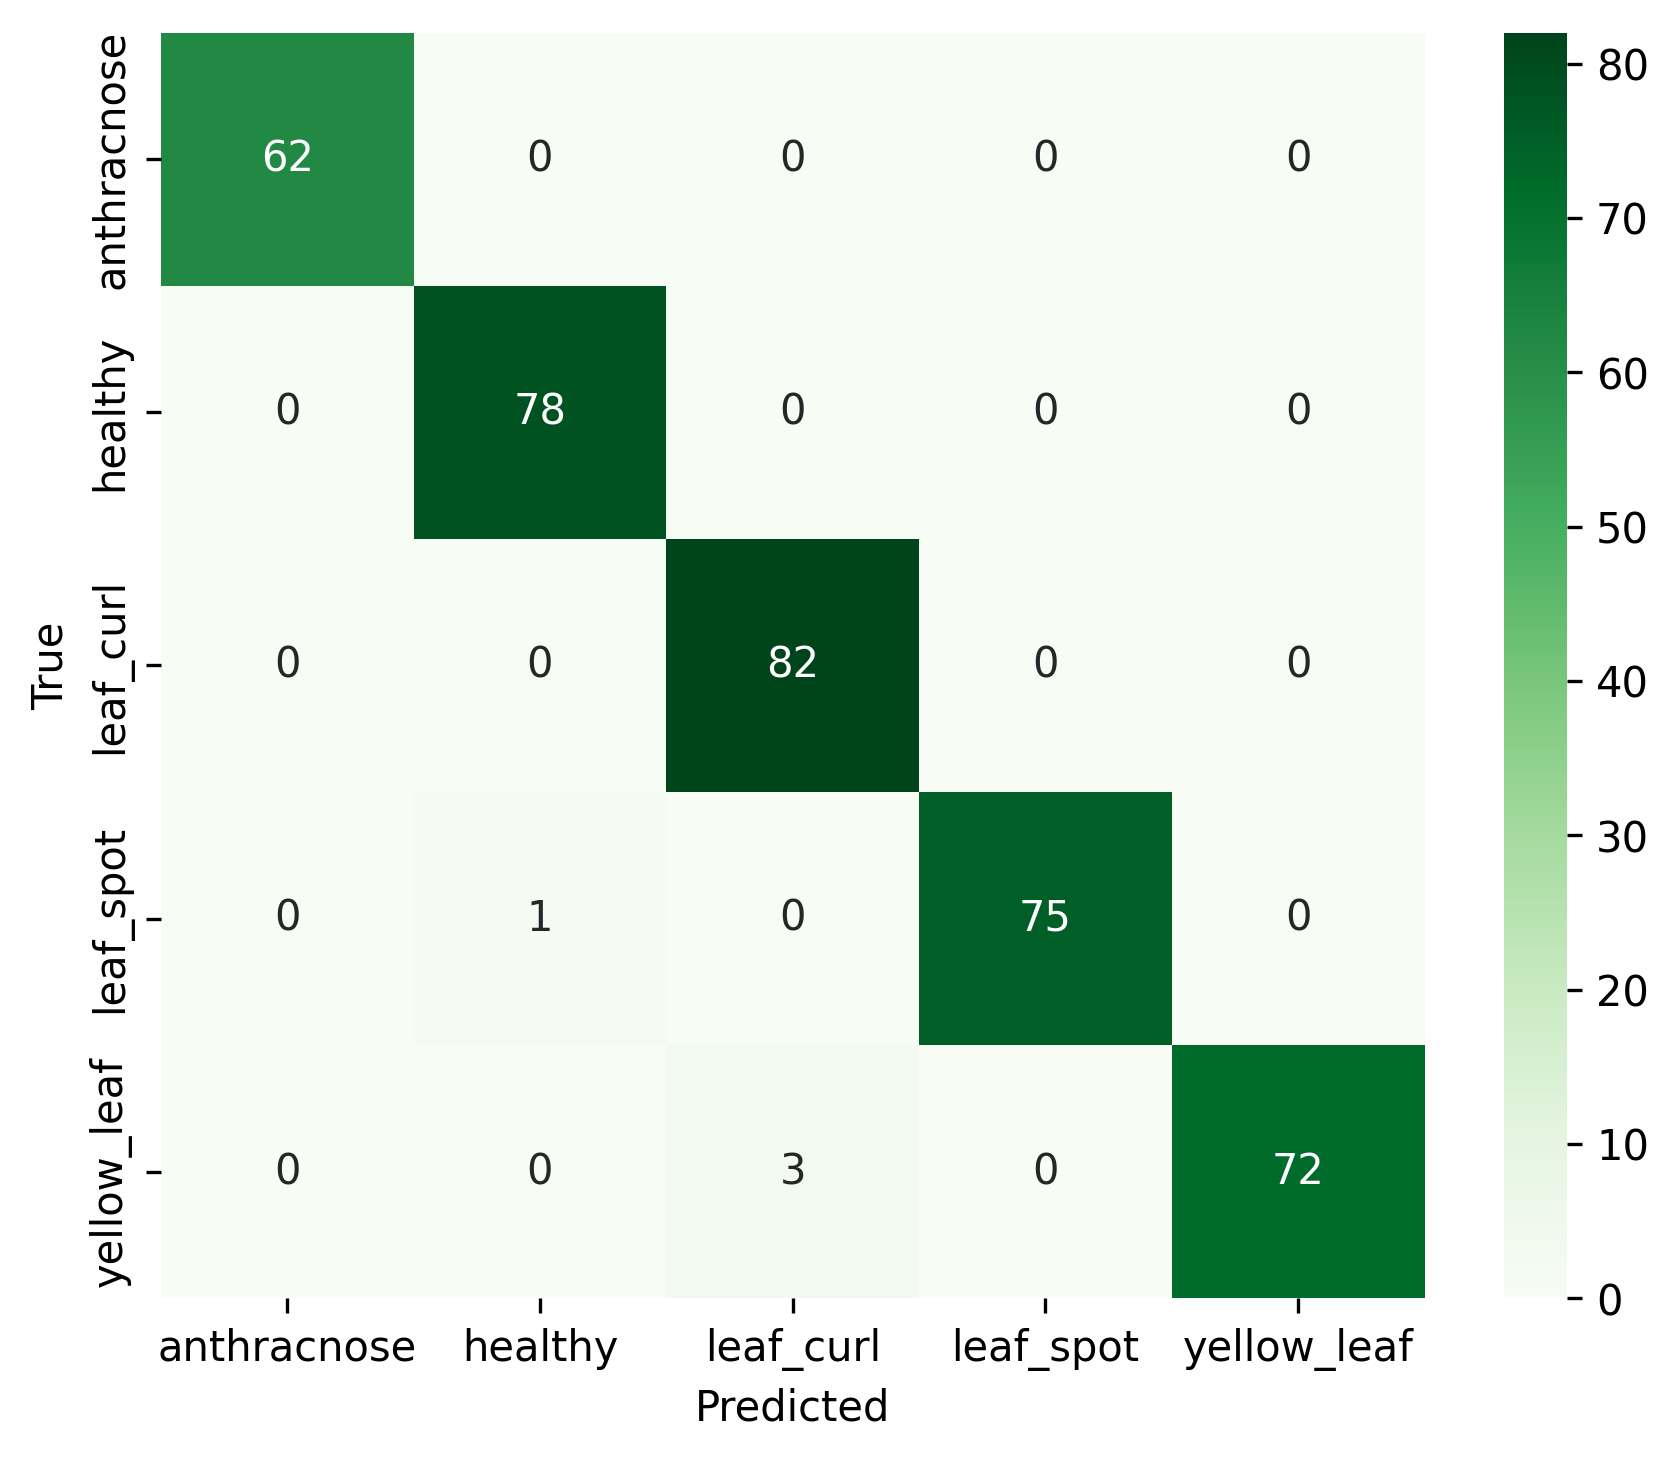
\includegraphics[width=0.8\linewidth,height=0.42\textheight,keepaspectratio]{figs/fig2.png}
\caption*{\textbf{Fig.\ 2.} Confusion matrix of ChiliEdgeNet on the test set (augmented scenario).}
\label{fig:2}
\end{figure*}

\subsection{Ablation Analysis}\label{ablation-analysis}

Every variant is retrained from scratch with seed 42, using the same data, training recipe, and 30 epochs. The current model contains neither Triplet Attention nor \emph{RES\_Block}. Since clean-image accuracy is already near saturation, the role of the Tiny Transformer is further examined with a multi-level stress test on synthetically degraded images.

\subsubsection{Block-Level Ablation}\label{block-level-ablation}

Two direct cuts respectively remove the Tiny Transformer and disable every skip connection of the \emph{InvertedResidual} blocks in the backbone. For Triplet Attention and \emph{RES\_Block}, this work uses a 2×2 add-back design: both present, only Triplet, only \emph{RES\_Block}, and neither (the current model).

\begin{table}[H]
\centering
\caption*{\textbf{Table 5.} Architectural ablation results on clean images, seed 42.}
\label{tab:5}
\small
\setlength{\tabcolsep}{3pt}
\renewcommand{\arraystretch}{1.15}
\begin{tabular}{lll}
\toprule
\textbf{Configuration} & \textbf{Parameters} & \textbf{Accuracy (\%)} \\
\midrule
\textbf{Current: no Triplet/RES\_Block} & \textbf{671,173} & \textbf{98.93} \\
Remove Tiny Transformer & 555,845 & 99.20 \\
Disable MobileNetV2 residuals & 671,173 & 96.51 \\
Add Triplet + RES\_Block & 671,732 & 97.59 \\
Triplet only & 671,473 & 98.12 \\
RES\_Block only & 671,432 & 98.93 \\
\bottomrule
\end{tabular}
\end{table}

\begin{table}[H]
\centering
\caption*{\textbf{Table 6.} McNemar test for the two direct cuts on clean images. Positive delta means the current model outperforms the variant; $p_{Holm}$ is corrected for two predefined contrasts.}
\label{tab:6}
\footnotesize
\setlength{\tabcolsep}{3pt}
\renewcommand{\arraystretch}{1.15}
\begin{tabular}{lllll}
\toprule
\textbf{Cut} & \textbf{Delta (pp)} & \textbf{b / c} & $p$ & \emph{\textbf{p\_Holm}} \\
\midrule
Remove Tiny Transformer & $-$0.27 & 0 / 1 & 1.0000 & 1.0000 \\
Disable MobileNetV2 residuals & +2.41 & 10 / 1 & 0.0117 & \textbf{0.0234} \\
\bottomrule
\end{tabular}
\end{table}

On clean images, the variant without the Transformer scores one image higher, so this run does not show the block's benefit (Table 5). In contrast, disabling the residual connections reduces net correct predictions by nine, and the difference remains significant after Holm correction (Table 6). This result supports keeping MobileNetV2's active skip branches.

\begin{table}[H]
\centering
\caption*{\textbf{Table 7.} Three contrasts removing Triplet Attention/RES\_Block from the both-present configuration. Holm-corrected $p$-values for three contrasts on clean images.}
\label{tab:7}
\small
\renewcommand{\arraystretch}{1.15}
\begin{tabular}{lll}
\toprule
\textbf{Contrast} & \textbf{Delta (pp)} & \emph{\textbf{p\_Holm}} \\
\midrule
Remove \emph{RES\_Block} & +0.54 & 0.625 \\
Remove Triplet Attention & +1.34 & 0.375 \\
Remove both, back to the current model & +1.34 & 0.375 \\
\bottomrule
\end{tabular}
\end{table}

No contrast reaches significance after Holm correction (Table 7). In this run, \emph{RES\_Block} alone gives the same accuracy as the current model, while Triplet Attention shows a trend toward lower performance. The results support removing both blocks to avoid unnecessary complexity, but do not prove the architectures are equivalent.

\subsubsection{Stress Test on the Role of the Tiny Transformer}\label{stress-test-on-the-role-of-the-tiny-transformer}

The stress test uses the same 373 test images and two seed-42 checkpoints: full ChiliEdgeNet and a variant retrained after removing the Tiny Transformer. Gaussian blur was generated with \emph{cv2.GaussianBlur} (\emph{sigmaX=0}) at kernel sizes 3, 5, 7, and 9; brightness reduction was generated by multiplying all pixel intensities by 0.8, 0.6, 0.4, and 0.2. Eight conditions were fixed before scoring. The clean image is only a reference point and is not part of the family of eight tests; Holm-corrected exact McNemar tests are applied across the eight degradation conditions.

\begin{figure*}[!tb]
\centering
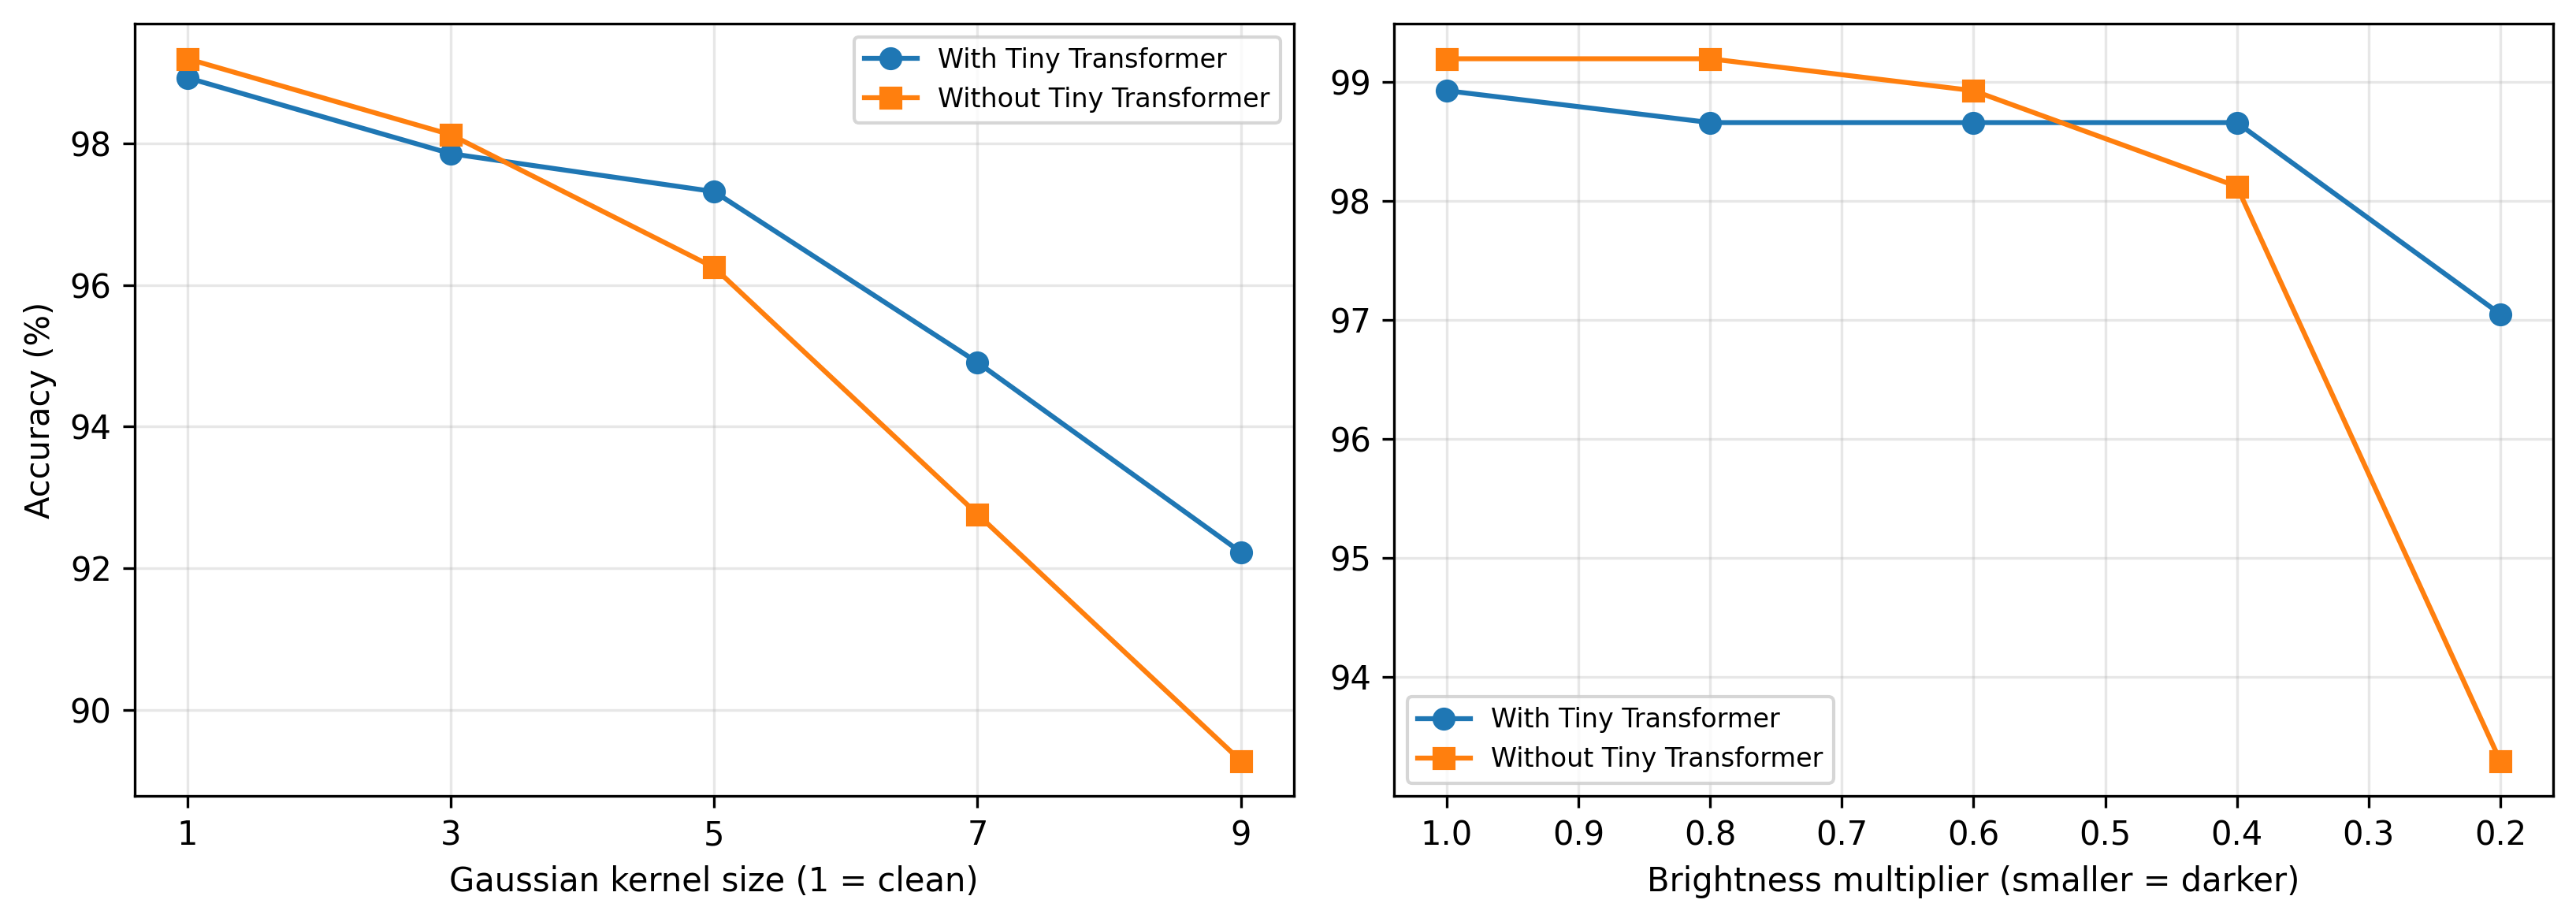
\includegraphics[width=0.8\linewidth,height=0.42\textheight,keepaspectratio]{figs/fig3.png}
\caption*{\textbf{Fig.\ 3.} Accuracy of ChiliEdgeNet with and without the Tiny Transformer across Gaussian blur levels and synthetic brightness-reduction factors.}
\label{fig:3}
\end{figure*}

\begin{table*}[!tb]
\centering
\caption*{\textbf{Table 8.} Stress test of the Tiny Transformer under synthetic degradation levels. Positive delta means the model with the Tiny Transformer performs better.}
\label{tab:8}
\footnotesize
\renewcommand{\arraystretch}{1.15}
\begin{tabular}{llllll}
\toprule
\textbf{Condition} & \textbf{With Transformer (\%)} & \textbf{Without Transformer (\%)} & \textbf{Delta (pp)} & \textbf{b / c} & \emph{\textbf{p\_Holm}} \\
\midrule
Clean & 98.93 & 99.20 & $-$0.27 & 0 / 1 & -- \\
Blur, kernel 3 & 97.86 & 98.12 & $-$0.27 & 2 / 3 & 1.0000 \\
Blur, kernel 5 & 97.32 & 96.25 & +1.07 & 6 / 2 & 1.0000 \\
Blur, kernel 7 & 94.91 & 92.76 & +2.14 & 15 / 7 & 0.8028 \\
Blur, kernel 9 & 92.23 & 89.28 & +2.95 & 22 / 11 & 0.5610 \\
Brightness × 0.8 & 98.66 & 99.20 & $-$0.54 & 0 / 2 & 1.0000 \\
Brightness × 0.6 & 98.66 & 98.93 & $-$0.27 & 1 / 2 & 1.0000 \\
Brightness × 0.4 & 98.66 & 98.12 & +0.54 & 3 / 1 & 1.0000 \\
Brightness × 0.2 & \textbf{97.05} & 93.30 & \textbf{+3.75} & 16 / 2 & \textbf{0.0105} \\
\bottomrule
\end{tabular}
\end{table*}

On clean images and mild degradation levels, the Tiny Transformer does not yet produce a clear difference. From kernel 5 onward, the advantage under blur grows with the degradation level (Fig. 3), but individual contrasts do not reach significance after Holm correction. At brightness factor 0.2, the full model reaches 97.05\%, 3.75 pp higher, reducing errors from 25 to 11; this is the only contrast that remains significant after correction (Table 8). These results suggest the Tiny Transformer helps maintain representations under severe visual degradation, rather than providing a stable advantage on clean images. This benefit comes with 115,328 additional parameters relative to the variant without the Transformer.

\subsubsection{Technique-Level Ablation}\label{technique-level-ablation}

Each variant replaces exactly one technique in the Tiny Transformer with its standard counterpart while keeping the remaining components unchanged.

\begin{table}[H]
\centering
\caption*{\textbf{Table 9.} Ablation of individual techniques in the Tiny Transformer on clean images, seed 42.}
\label{tab:9}
\footnotesize
\setlength{\tabcolsep}{3pt}
\renewcommand{\arraystretch}{1.15}
\begin{tabular}{llll}
\toprule
\textbf{Variant} & \textbf{Replaced component} & \textbf{Parameters} & \textbf{Accuracy (\%)} \\
\midrule
\textbf{ChiliEdgeNet} & 2D-RoPE + GQA + RMSNorm & \textbf{671,173} & \textbf{98.93} \\
\emph{learned\_pe} & 2D-RoPE → learned PE & 696,261 & 98.93 \\
\emph{mha} & GQA → MHA & 687,557 & 98.93 \\
\emph{layernorm} & RMSNorm → LayerNorm & 671,557 & 98.39 \\
\bottomrule
\end{tabular}
\end{table}

On clean images (Table 9), learned PE and MHA give the same correct/incorrect predictions as ChiliEdgeNet; LayerNorm is lower by two images, but McNemar shows no significance ($p = 0.5$). The three choices---2D-RoPE, GQA, and RMSNorm---are not shown by this single-seed data to be superior in accuracy. In terms of parameter structure, they respectively avoid 25,088, 16,384, and 384 parameters relative to the standard alternatives, totalling 41,856 parameters if all three standard alternatives were used simultaneously; the combined three-replacement variant has not been separately trained.

\subsection{Model Interpretability}\label{model-interpretability}

The analyses in this section use ChiliEdgeNet's original checkpoint, trained only on ChiliEdge-DS and used to produce the in-domain results in Table 4. The augmented checkpoint used for the domain-transfer experiment in Section 4.5 is a separate adapted model and is not used to produce the interpretability results below.

\subsubsection{Explainable AI (XAI)}\label{explainable-ai-xai}

High accuracy alone is not sufficient to interpret model behaviour, particularly since ChiliEdge-DS predominantly uses a controlled white background. This work applies three complementary XAI methods on the ChiliEdgeNet augmented-scenario checkpoint (seed 42), each using one representative image per class. Gradient SHAP \cite{erion2021} estimates pixel contribution from gradients relative to a baseline distribution; Occlusion Sensitivity \cite{zeiler2014} occludes 32×32-pixel regions in turn and measures the change in output; Attention Rollout \cite{abnar2020} aggregates attention flow through the Transformer block across the full 14×14 grid. Because the architecture uses mean pooling and has no \emph{CLS} token, the Rollout map is produced by averaging attention flow across the 196 tokens, rather than tracing from a single output token.

The three maps offer distinct perspectives: Occlusion shows region-level sensitivity (Fig. 4); Gradient SHAP gives pixel-level attribution distributed over the object surface (Fig. 5); Attention Rollout reflects the Transformer's internal attention propagation (Fig. 6). Across the five illustrative images, high-response regions generally intersect with the leaf/fruit or the diseased area, though the degree of concentration differs across methods and classes. Since the evaluation uses only one image per class and no ground-truth symptom segmentation exists, this result is an exploratory qualitative survey only; it does not prove the model has learned correct pathological features, fully ignored the background, or captured a genuine causal relationship. The 14×14 grid provides 196 spatial positions, four times more than a 7×7 grid, giving the Rollout map finer visual resolution.

\begin{figure*}[!tb]
\centering
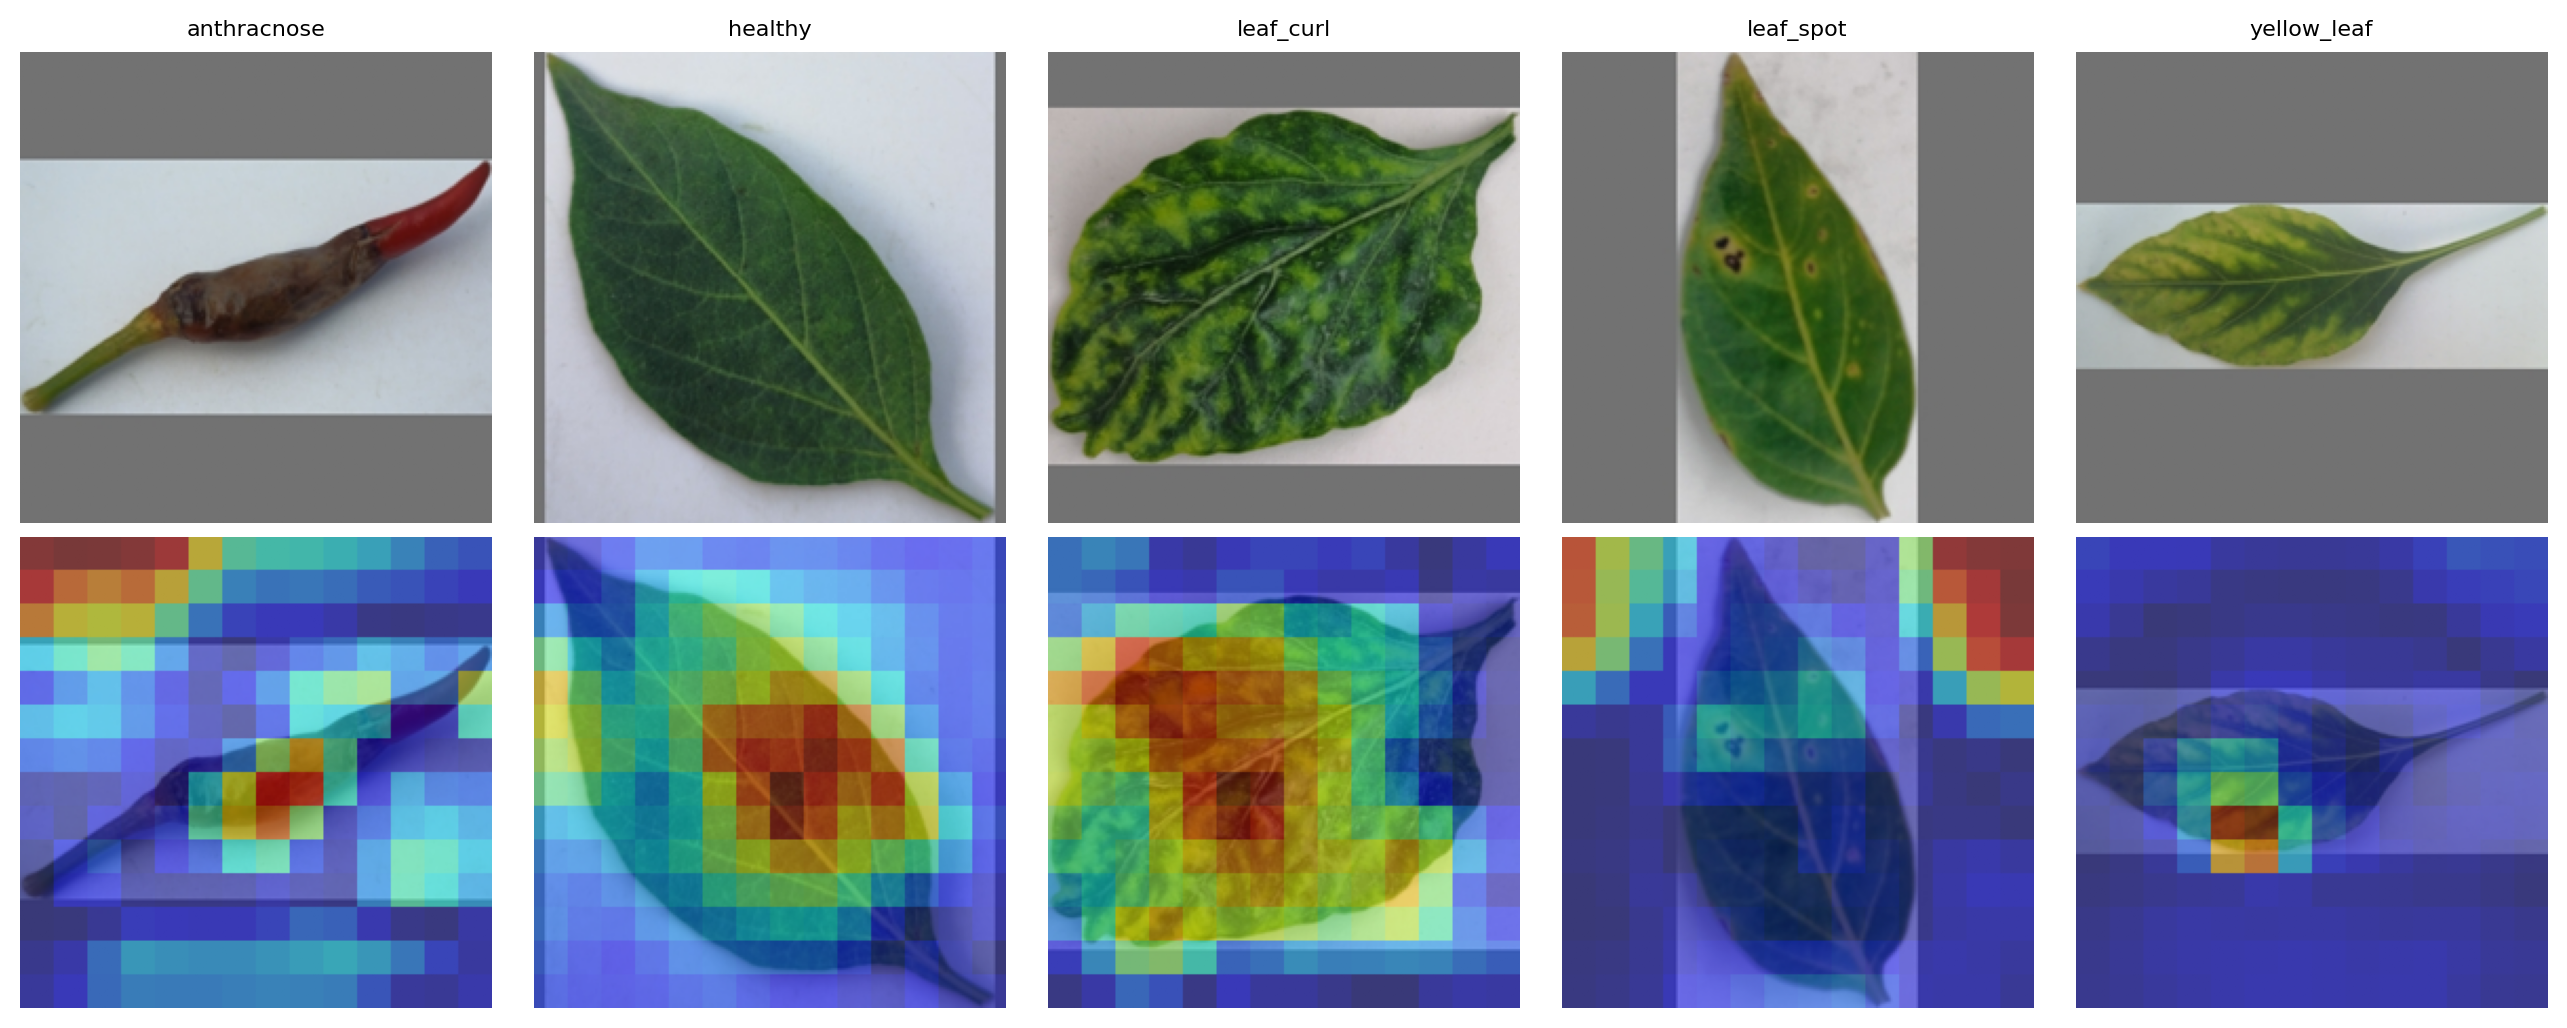
\includegraphics[width=0.8\linewidth,height=0.42\textheight,keepaspectratio]{figs/fig4.png}
\caption*{\textbf{Fig.\ 4.} Occlusion Sensitivity for the five disease classes (top: original image; bottom: sensitivity map overlay). Bright regions are where occlusion costs the model the most confidence; this technique treats the model as a black box.}
\label{fig:4}
\end{figure*}

\begin{figure*}[!tb]
\centering
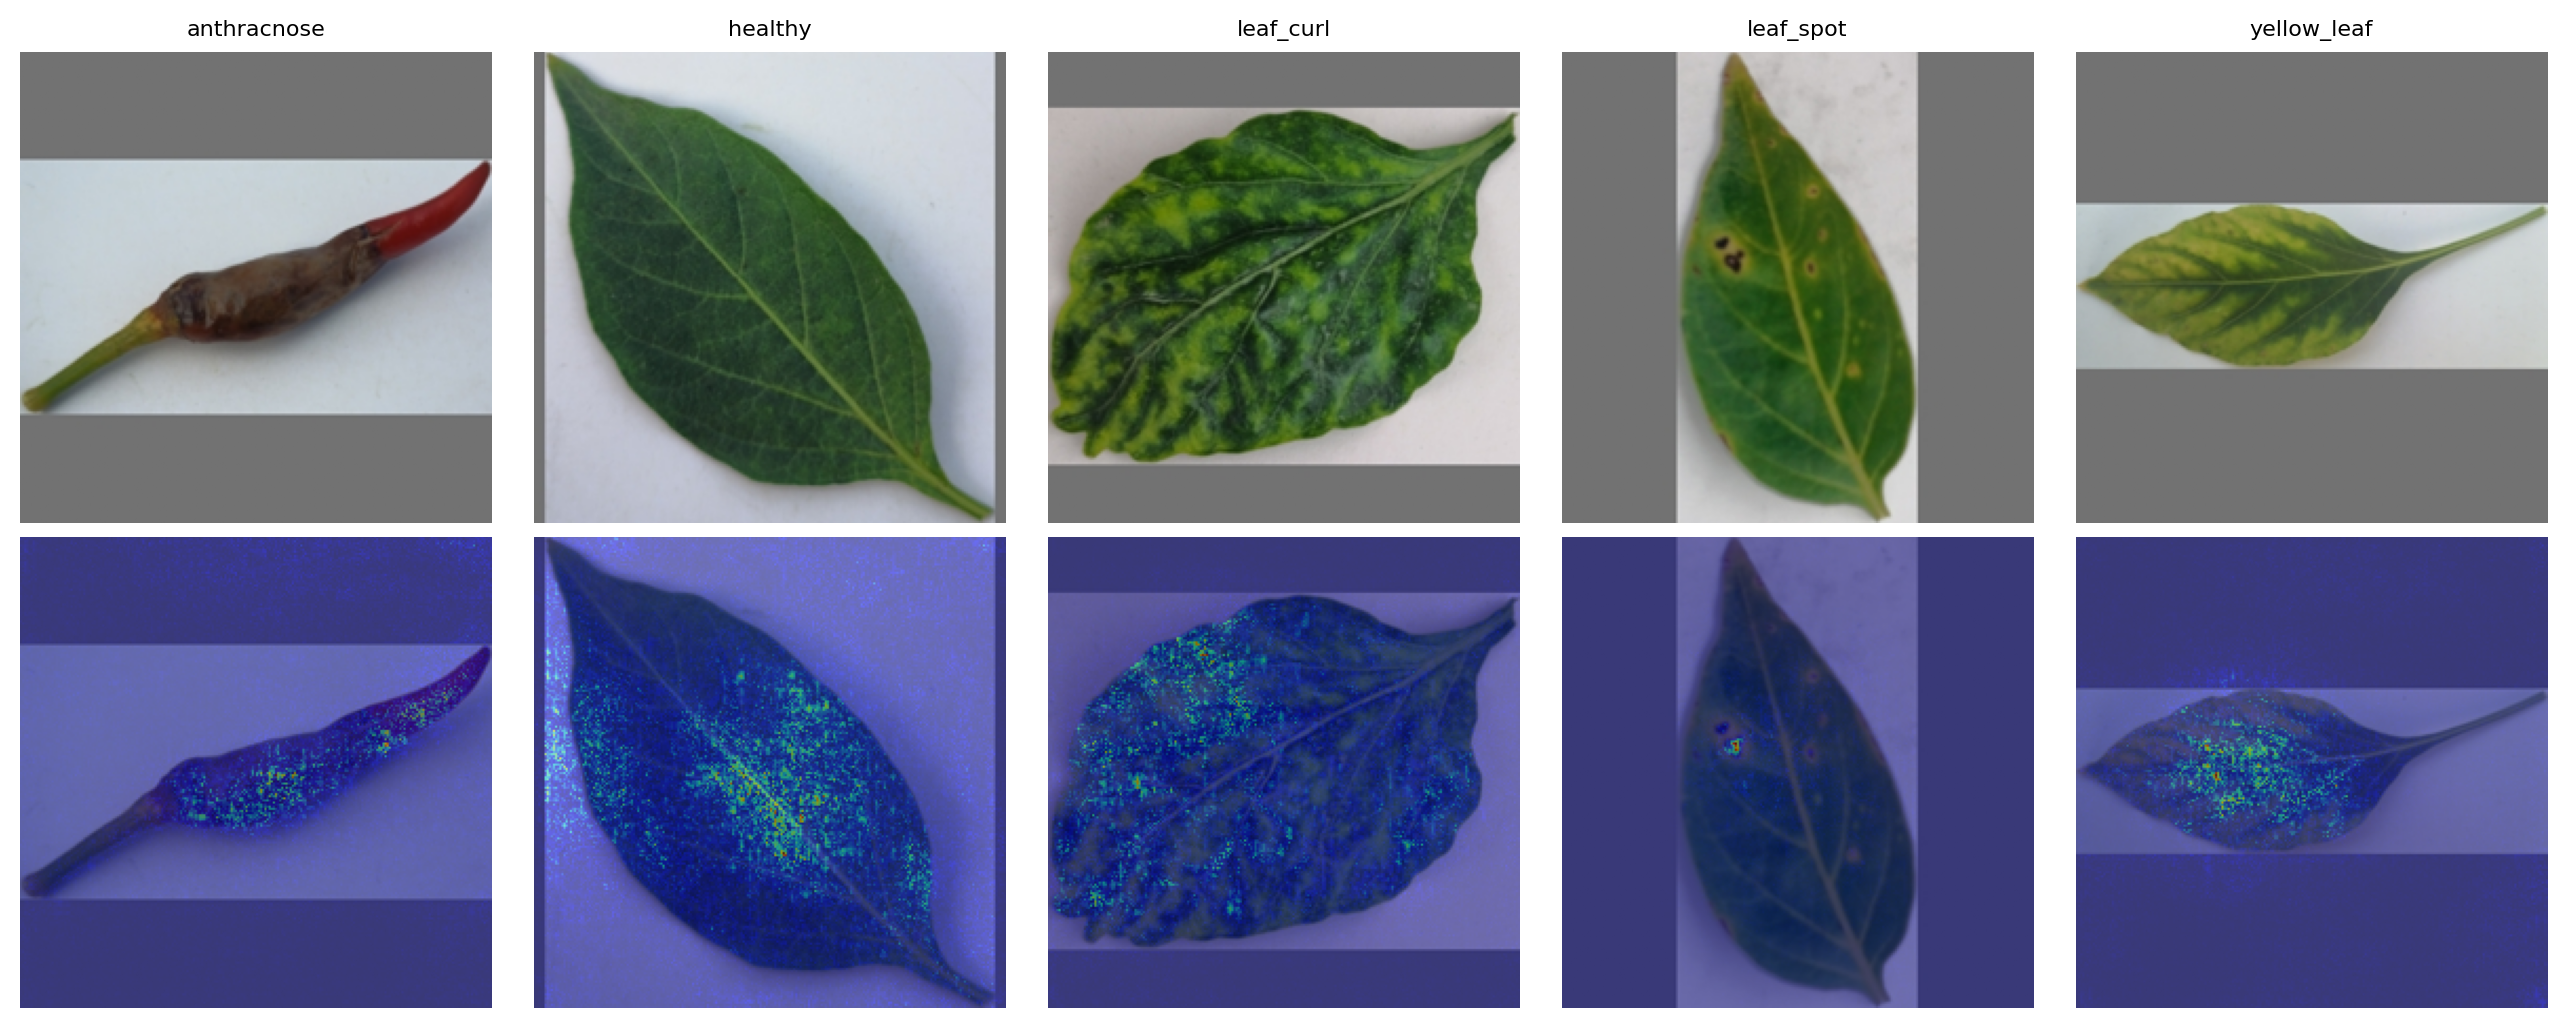
\includegraphics[width=0.8\linewidth,height=0.42\textheight,keepaspectratio]{figs/fig5.png}
\caption*{\textbf{Fig.\ 5.} Gradient SHAP for the five classes (top: original image; bottom: pixel-attribution magnitude overlay), computed with 20 samples and two constant baseline tensors (0 and 1) in the normalized input space.}
\label{fig:5}
\end{figure*}

\begin{figure*}[!tb]
\centering
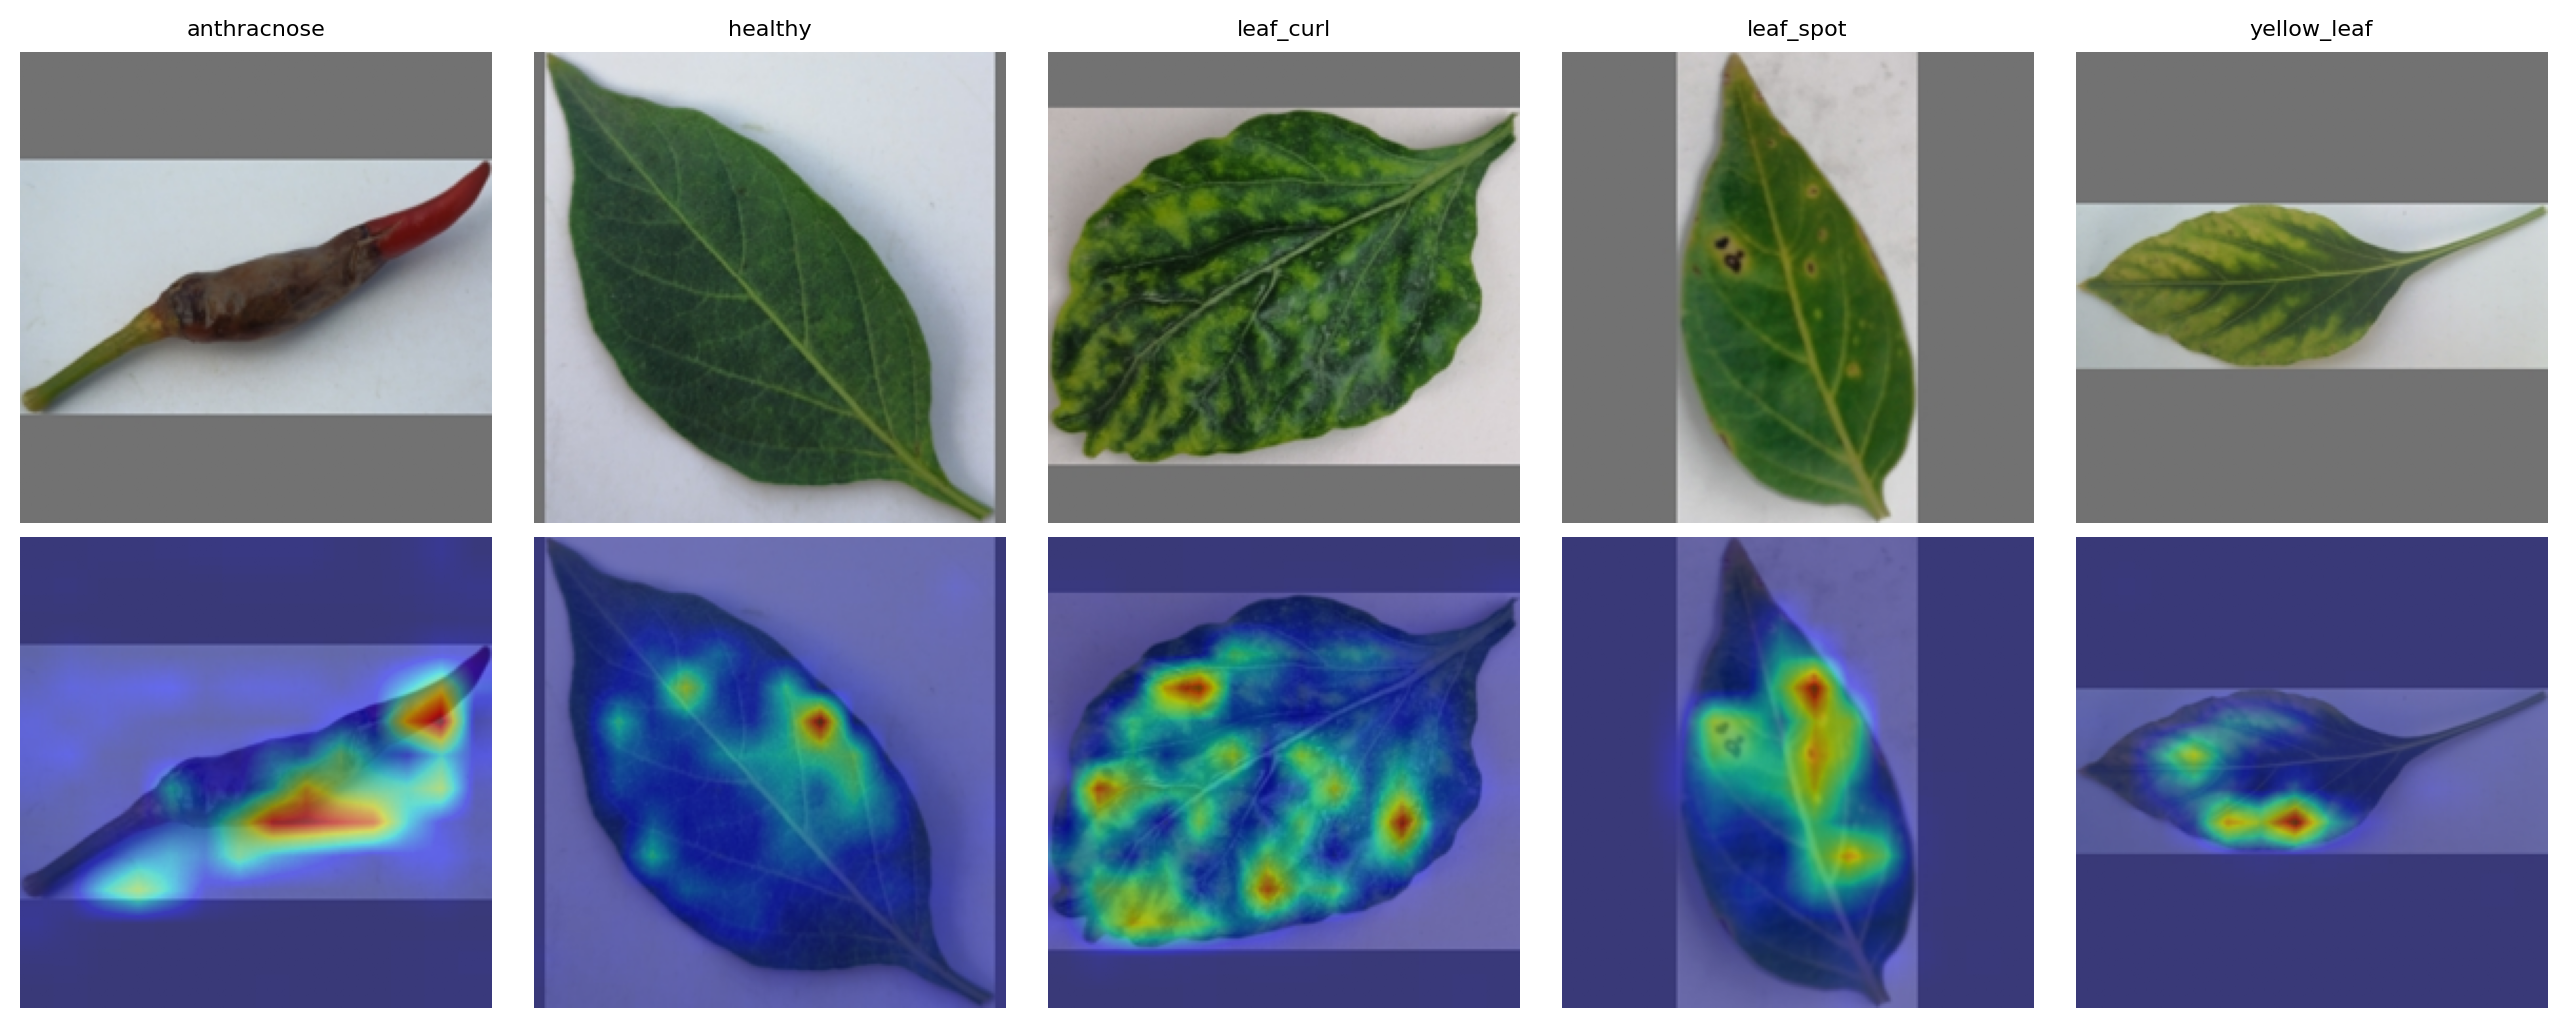
\includegraphics[width=0.8\linewidth,height=0.42\textheight,keepaspectratio]{figs/fig6.png}
\caption*{\textbf{Fig.\ 6.} Attention Rollout of the Tiny Transformer block on the 14×14 grid, aggregated by averaging attention flow across the 196 tokens since the model uses mean pooling with no \emph{CLS} token.}
\label{fig:6}
\end{figure*}

\subsubsection{Comparison with a General-Purpose Multimodal Model}\label{comparison-with-a-general-purpose-multimodal-model}

This work uses the general-purpose multimodal model Gemini 3.1 Flash Lite, API model ID \emph{gemini-3.1-flash-lite}, accessed on 8 July 2026 \cite{googledeepmind2026} with default generation settings to classify the raw images directly in a zero-shot setting. The model was prompted, in Vietnamese, to classify each image into exactly one of the five ChiliEdge-DS labels; the \emph{predicted\_class} field is scored directly against these five strings, with no synonym translation or post-hoc mapping. All 373 API calls returned valid, parseable output, with no exclusions. The exact prompt text is preserved in the study's accompanying materials rather than reproduced here, since this is a secondary reference comparison, not the paper's main contribution: Gemini was not fine-tuned on ChiliEdge-DS, whereas ChiliEdgeNet is a specialized classifier trained with supervision for exactly the five classes.

As summarized in Table 10, Gemini reaches 78.55\% accuracy, while ChiliEdgeNet reaches 98.93\% on the same 373-image test set, matching Table 4. Of the three \emph{yellow\_leaf} images misclassified by ChiliEdgeNet as \emph{leaf\_curl} (Section 4.2), Gemini correctly classified all three as \emph{yellow\_leaf}.

\textbf{On latency.} The approximately 105x figure contrasts 20.24 ms of local inference with a 2,123 ms median cloud API round-trip. The two figures are not equivalent: the round-trip includes network latency, server-side queueing, and provider-side batching---none of which is computation intrinsic to the model. This is a comparison between two deployment modes, not a claim that one architecture computes roughly 105x faster than the other. Similarly, although accuracy is computed on the same 373 images, the accuracy gap does not constitute a peer comparison. The commercial endpoint may also be updated over time, so this comparison is reproducible only against the stated model ID, prompt, and access date.

\begin{table}[H]
\centering
\caption*{\textbf{Table 10.} Comparison of ChiliEdgeNet with Gemini 3.1 Flash Lite on the full 373-image test set (accessed 8 July 2026).}
\label{tab:10}
\footnotesize
\renewcommand{\arraystretch}{1.15}
\begin{tabular}{lll}
\toprule
\textbf{System} & \textbf{Accuracy} & \textbf{Latency/image} \\
\midrule
\textbf{ChiliEdgeNet (local CPU)} & \textbf{98.93\%} & \textbf{20.24 ms} \\
Gemini 3.1 Flash Lite (\emph{gemini-3.1-flash-lite}) & 78.55\% & 2,123 ms \\
\bottomrule
\end{tabular}
\end{table}

\subsection{Four-Class Cross-Dataset Evaluation After Few-Shot Adaptation}\label{four-class-cross-dataset-evaluation-after-few-shot-adaptation}

The stress tests in Section 4.3 only synthesize blur and brightness reduction from ChiliEdge-DS images, so they do not fully capture the acquisition domain gap. This work carries out an additional evaluation on the Chili Plant Leaf Disease and Growth Stage Dataset from Bangladesh, version 1, released on Mendeley Data under a CC BY 4.0 licence \cite{nirob2025}. The source images were collected at a garden in Charpolisha, Jamalpur (Bangladesh) between October 2024 and February 2025; the disease-leaf portion comprises 1,856 images across six source labels. Cross-domain robustness under few-shot adaptation has also been studied through target-domain statistical calibration \cite{zhao2026} and laboratory-to-field transfer for crop disease identification \cite{yangS2024}; the evaluation here follows a similar motivation but is restricted to the chili-specific four-class mapping described below.

Only four labels with a direct correspondence to the ChiliEdgeNet label space are used. Two labels, \emph{Bacterial Spot} (156 images) and \emph{White spot} (195 images), are excluded because the model has no corresponding target class. The source dataset has no anthracnose class, so there is no \emph{anthracnose} ground-truth row. However, the checkpoint still retains all five outputs used during training; any prediction toward \emph{anthracnose} is still counted as incorrect, and this prediction column is kept in the confusion matrix.

\begin{table*}[!tb]
\centering
\caption*{\textbf{Table 11a.} Verified support/query split from the four mapped classes.}
\label{tab:11a}
\footnotesize
\setlength{\tabcolsep}{2.5pt}
\renewcommand{\arraystretch}{1.15}
\begin{tabular}{llllll}
\toprule
\textbf{Source label \cite{nirob2025}} & \textbf{ChiliEdgeNet label} & \textbf{Original} & \textbf{Support} & \textbf{Clean query} & \textbf{Corrected test} \\
\midrule
\emph{Healthy Leaf} & \emph{healthy} & 458 & 8 & 450 & 450 \\
\emph{Curl Virus} & \emph{leaf\_curl} & 423 & 9 & 414 & 414 \\
\emph{Cercospora Leaf Spot} & \emph{leaf\_spot} & 180 & 16 & 164 & 164 \\
\emph{Nutrition Deficiency} & \emph{yellow\_leaf} & 444 & 9 & 435 & 435 \\
\textbf{Total} & & \textbf{1,505} & \textbf{42} & \textbf{1,463} & \textbf{1,463} \\
\bottomrule
\end{tabular}
\end{table*}

\begin{table*}[!tb]
\centering
\caption*{\textbf{Table 11b.} Results before and after few-shot adaptation on the 1,463-image clean query set.}
\label{tab:11b}
\footnotesize
\setlength{\tabcolsep}{2pt}
\renewcommand{\arraystretch}{1.15}
\begin{tabular}{lllllll}
\toprule
\textbf{Configuration} & \textbf{Seed} & \textbf{Accuracy} & \textbf{Prec.-macro} & \textbf{Recall-macro} & \textbf{F1-macro} & \textbf{Correct} \\
\midrule
Original checkpoint & 42 & 30.96\% & 0.4337 & 0.2843 & 0.1766 & 453/1,463 \\
After few-shot & 42 & 89.75\% & 0.8837 & 0.8683 & 0.8744 & 1,313/1,463 \\
\textbf{Difference} & & \textbf{+58.78 pp} & \textbf{+0.4500} & \textbf{+0.5840} & \textbf{+0.6978} & \textbf{+860} \\
\bottomrule
\end{tabular}
\end{table*}

\begin{figure*}[!tb]
\centering
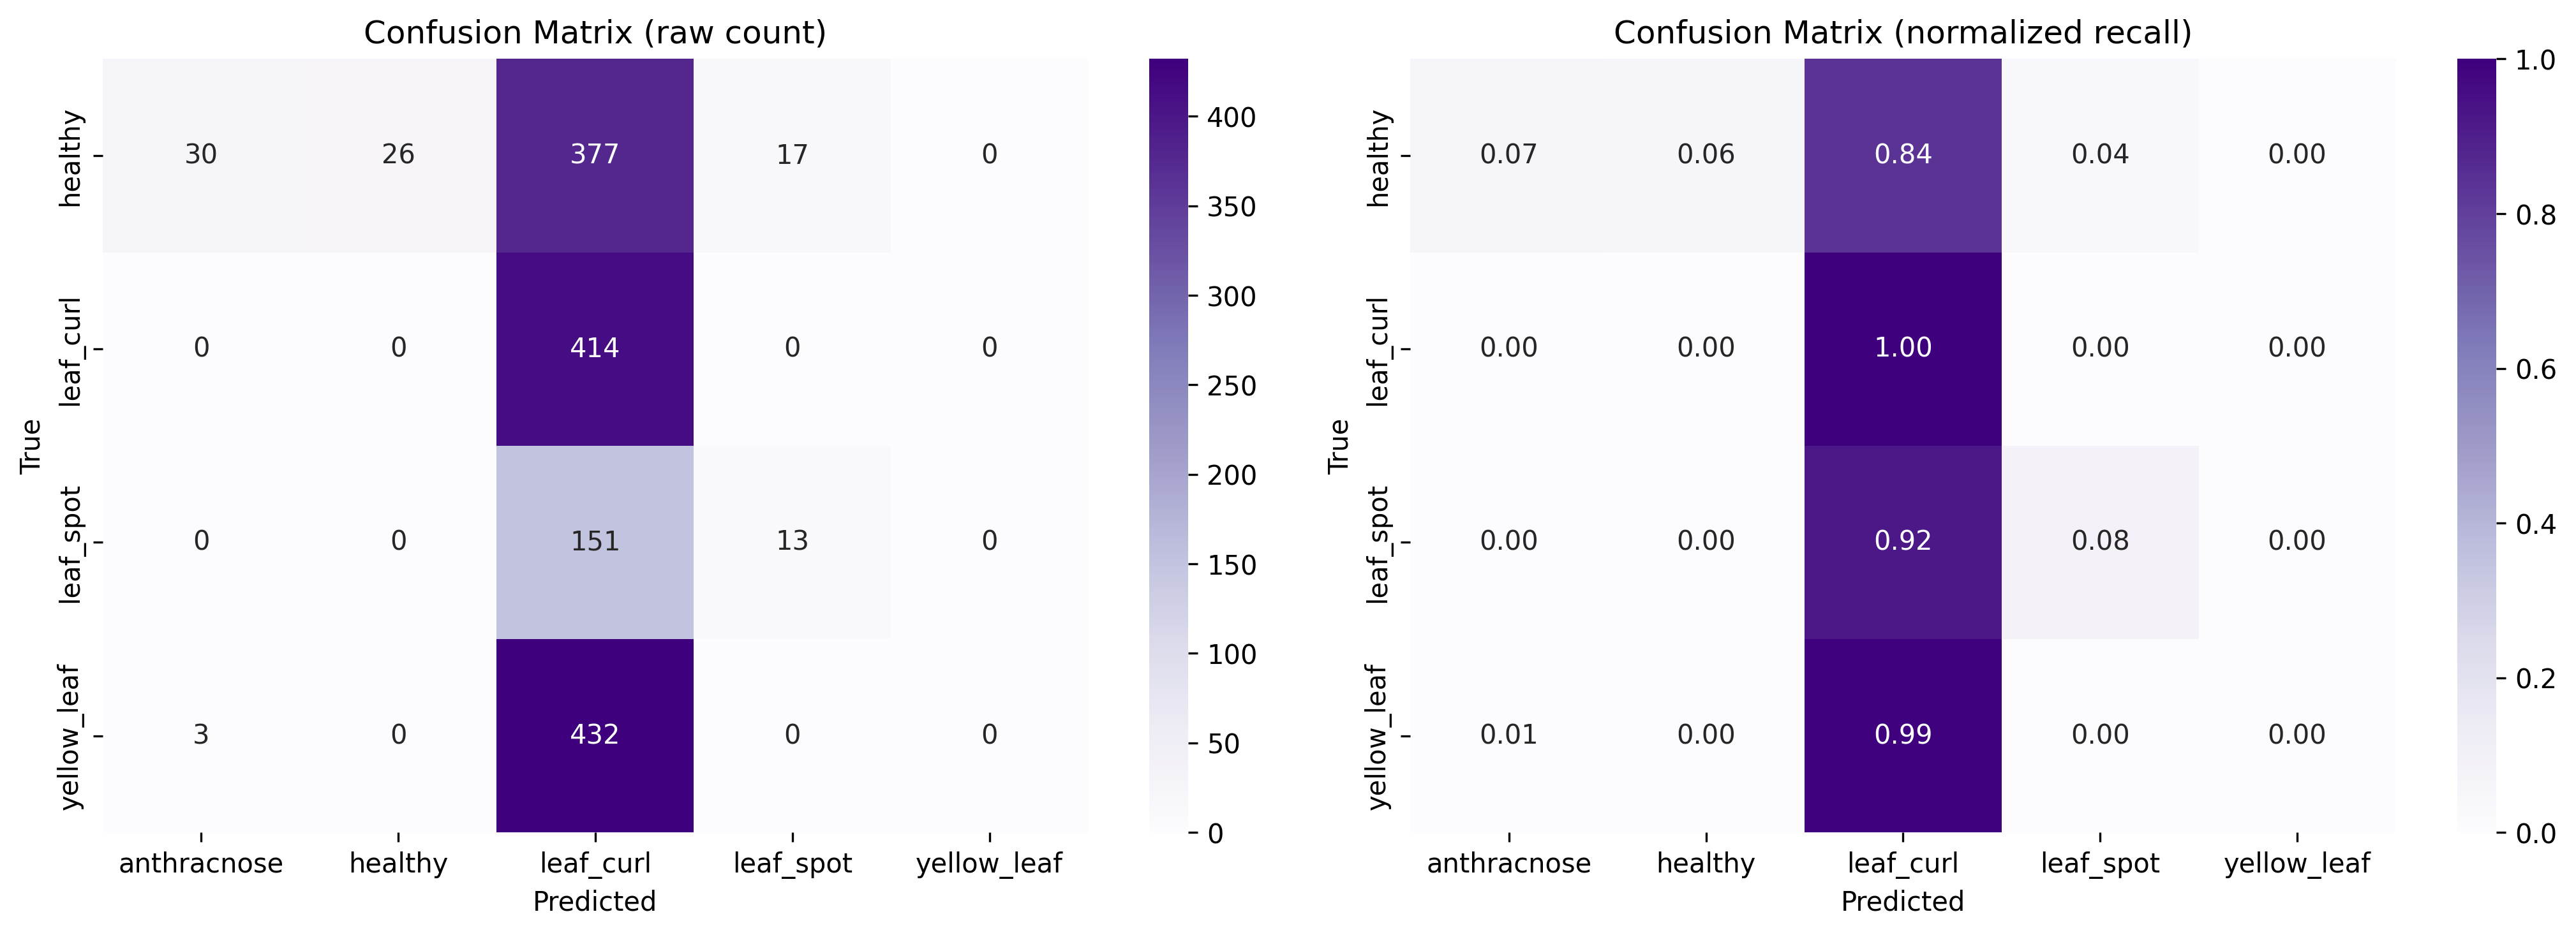
\includegraphics[width=0.8\linewidth,height=0.42\textheight,keepaspectratio]{figs/fig7.png}
\caption*{\textbf{Fig.\ 7.} Confusion matrix of the original checkpoint on the 1,463-image clean query set.}
\label{fig:7}
\end{figure*}

\begin{figure*}[!tb]
\centering
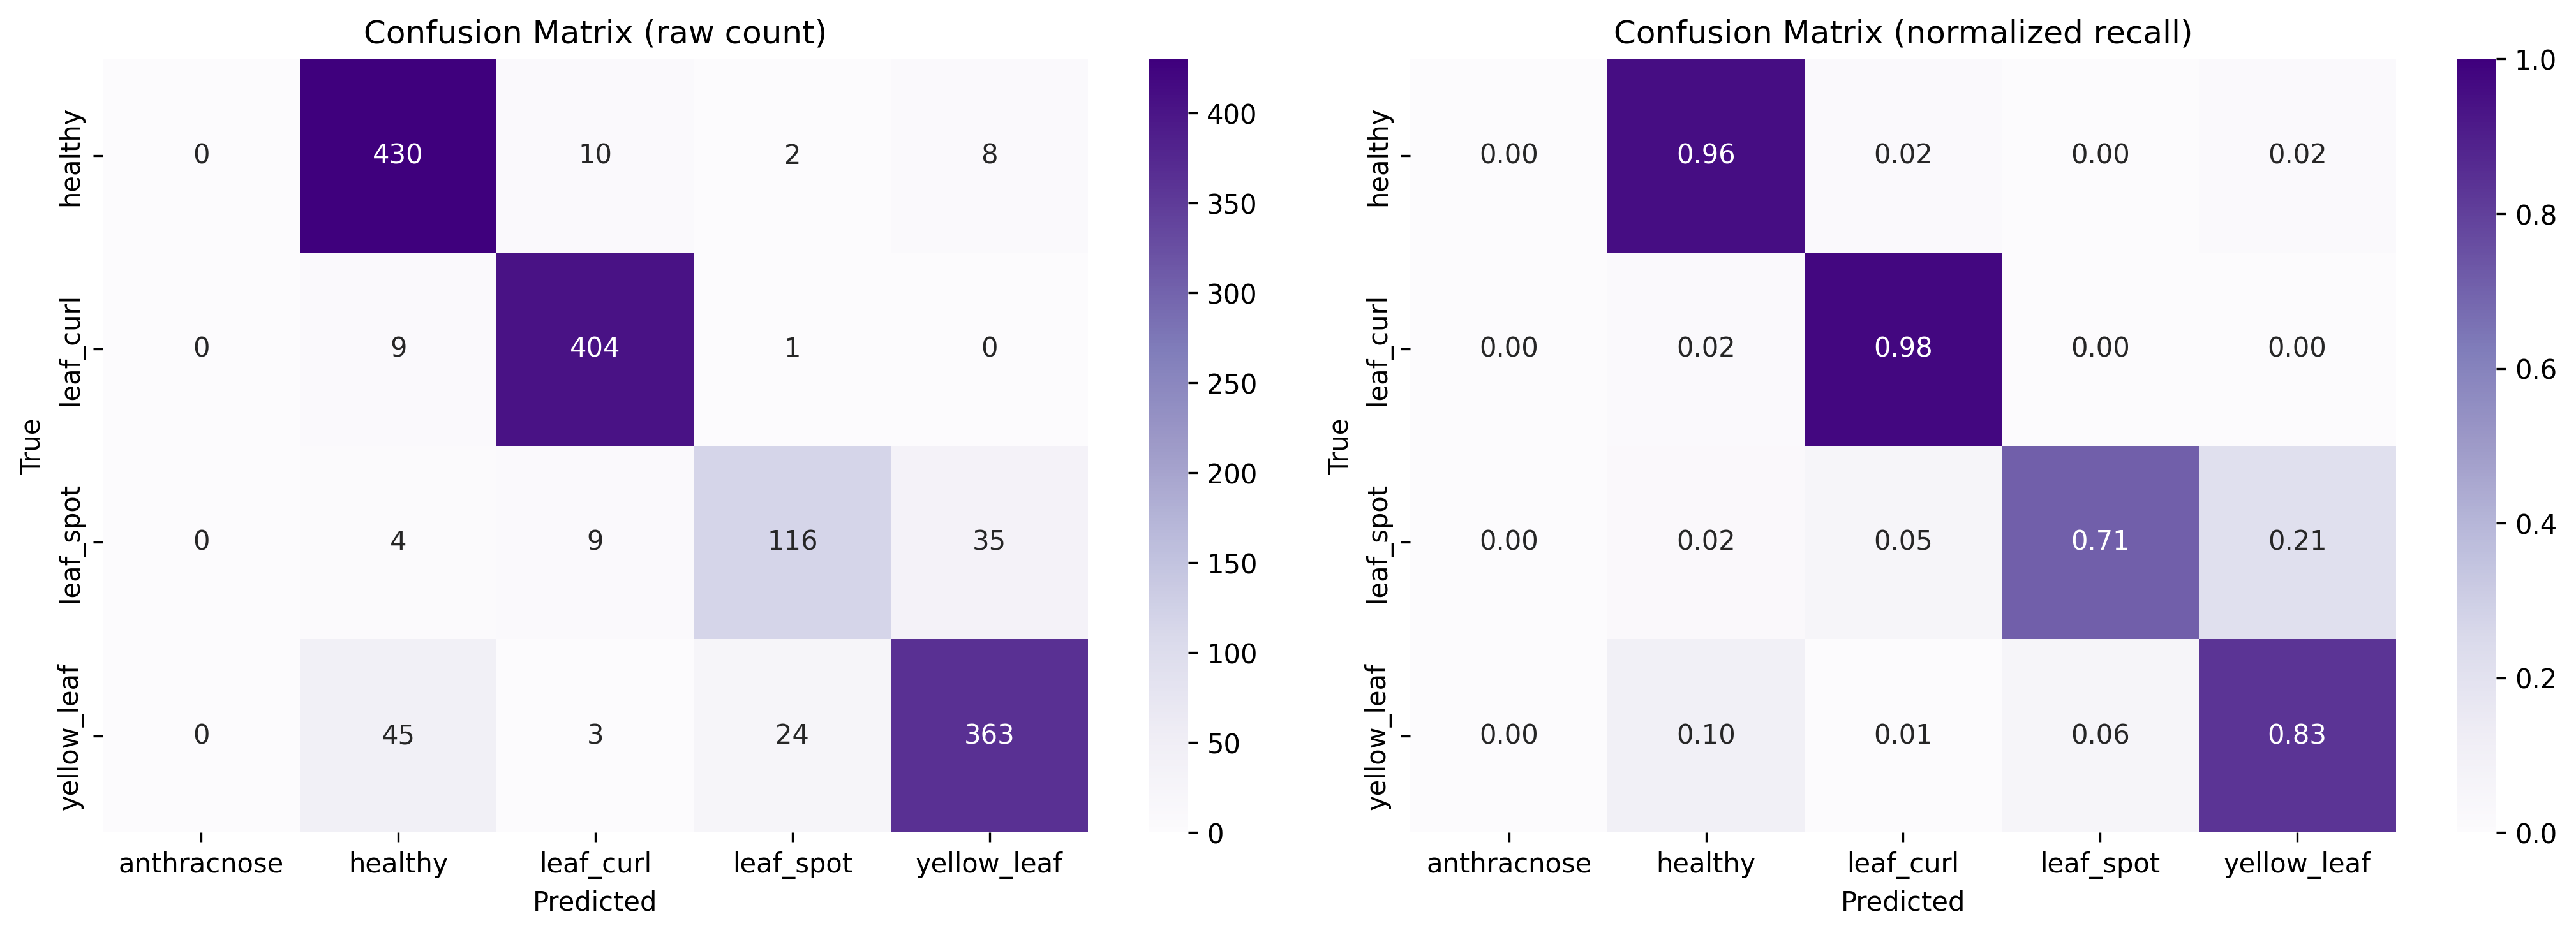
\includegraphics[width=0.8\linewidth,height=0.42\textheight,keepaspectratio]{figs/fig8.png}
\caption*{\textbf{Fig.\ 8.} Confusion matrix of the checkpoint after few-shot adaptation on the same 1,463-image clean query set.}
\label{fig:8}
\end{figure*}

\textbf{Few-shot setup.} The support set comprises 42 images taken as-is from Nirob et al. \cite{nirob2025}: 8 \emph{healthy}, 9 \emph{leaf\_curl}, 16 \emph{leaf\_spot}, and 9 \emph{yellow\_leaf} (Table 11a). The support images were added to ChiliEdge-DS's training set to create a separate adapted checkpoint; ChiliEdge-DS's own in-domain validation and test sets are unchanged. This is supervised domain adaptation with a small support set, not episodic meta-learning. The number of shots differs across classes, so this is not a balanced \emph{N}-way \emph{K}-shot setup.

To control for data leakage, the support and query sets were tracked with SHA-256 hashes rather than filenames alone. The query set is defined as the complement of the 42 support images within the 1,505 images across the four classes, and an audit confirmed the hash intersection between the two is zero. The few-shot checkpoint was trained with seed 42.

To support independent reproduction, the clean 1,463-image query set is released as the Chili Leaf Disease Cross-Dataset Query Set, Kaggle version 2 \cite{to2026a}, and the 42 support images are released as Chili Leaf Disease Few-Shot, Kaggle version 1 \cite{to2026b}. Both packages are derived splits of the original Mendeley Data dataset and do not replace the requirement to cite the source dataset \cite{nirob2025}.

\textbf{Results on the clean query set.} Both checkpoints were evaluated on the same 1,463-image clean query set (Table 11b). The original checkpoint uses seed 42 (SHA-256 verified); the checkpoint after few-shot adaptation also uses seed 42 (SHA-256 verified). Images were resized to 224×224 pixels and normalized with ImageNet statistics. Macro precision, recall, and F1 are averaged only over the four classes with ground truth; predictions toward \emph{anthracnose} still reduce accuracy.

At the original checkpoint, \emph{leaf\_curl} has recall 1.0000 but precision only 0.3013, while \emph{yellow\_leaf} has recall zero (Fig. 7). After few-shot adaptation, F1 for \emph{healthy}, \emph{leaf\_curl}, \emph{leaf\_spot}, and \emph{yellow\_leaf} reaches 0.9168, 0.9619, 0.7557, and 0.8633 respectively (Fig. 8). A per-image prediction comparison shows 443 images correctly predicted by both checkpoints, 140 images incorrectly predicted by both, 870 images turning from incorrect at the original checkpoint to correct after few-shot, and 10 images in the opposite direction. A two-sided exact McNemar test gives $p = 1.83 \times 10^{-242}$. This is a single paired contrast on an out-of-domain dataset and does not belong to the ablation's Holm test family. Predictions for all 1,463 images and the paired statistics are stored in the metadata package accompanying this study.

\subsection{Preprocessing and Inference Latency Evaluation in a Laptop-Camera Application}\label{preprocessing-and-inference-latency-evaluation-in-a-laptop-camera-application}

ChiliEdgeNet was integrated into a laptop camera application, where the user places a leaf inside a region of interest (ROI) and triggers a prediction on each frame. This experiment evaluates only preprocessing and inference latency as a proof of integration feasibility; it does not use camera frames to estimate real-field accuracy.

The test session comprises 62 predictions, run at batch size 1 on a 13th Gen Intel Core i7-13650HX CPU. The measured interval starts from converting the ROI's RGB image to PIL, continuing through resize, normalization, model inference, softmax, and top-1 prediction. The measurement excludes time for reading frames from the camera, cropping the ROI, converting BGR to RGB, rendering the UI, or writing files.

\begin{table}[H]
\centering
\caption*{\textbf{Table 12.} Preprocessing and inference latency of ChiliEdgeNet on a laptop CPU.}
\label{tab:12}
\small
\renewcommand{\arraystretch}{1.15}
\begin{tabular}{ll}
\toprule
\textbf{Metric} & \textbf{Latency (ms)} \\
\midrule
Number of measurements & 62 \\
Mean & 32.18 \\
Median & 29.70 \\
95th percentile & 46.49 \\
Minimum & 17.33 \\
Maximum & 122.76 \\
\bottomrule
\end{tabular}
\end{table}

A median of 29.70 ms and a 95th percentile of 46.49 ms show that the preprocessing-and-inference stage can respond quickly on a laptop CPU without a GPU (Table 12). However, the results come from a single measurement session on a single device and do not include the application's full capture-to-display cost; the test device is also not dedicated edge hardware. This experiment therefore provides only preliminary evidence of ChiliEdgeNet's feasibility for integration into a camera application, not a representative measurement of the full pipeline or of dedicated edge hardware. The labelled data in the demo session is unbalanced and contains many repeated frames of the same subject, so accuracy and a confusion matrix are not reported in this section.

\FloatBarrier

\section{Limitations}\label{limitations}

\textbf{Statistical resolution of the test set.} With 373 images, one image is worth 0.27 pp, and the proposed model errs on 4 images. The 0.80 pp (3-image) difference from the base architecture \cite{duhan2025} falls within the noise band of a single split: ChiliEdgeNet's 95\% Wilson interval {[}97.28, 99.58{]} overlaps with the {[}96.18, 99.09{]} interval of Duhan et al. \cite{duhan2025}. Both models are seed-42-matched but each has only been run once. Furthermore, RTR\_Lite\_MobileNet \cite{duhan2025} was chosen as the primary baseline after reviewing the baseline pool's test results, so this comparison is exploratory and does not constitute an independent test evaluation. Establishing a definitive ranking would require selection by validation followed by a single test evaluation, multiple seeds, and/or a direct McNemar test between the two prediction sets. The 35\% parameter reduction does not depend on training noise or baseline-selection criteria.

\textbf{Run count and statistical power.} The proposed model and all ablations come from a single seed-42 run. At the architectural level, disabling MobileNetV2 residuals reduces accuracy by 2.41 pp on clean images, and the difference remains significant after Holm correction for the two direct cuts ($p_{Holm} = 0.0234$). Across the eight stress-test conditions, the Tiny Transformer's advantage reaches significance after Holm correction only at brightness factor 0.2 ($p_{Holm} = 0.0105$); the remaining levels reflect a severity-dependent trend rather than a broadly established effect. All three Triplet/\emph{RES\_Block} contrasts are non-significant after Holm correction. These conclusions are single-seed observations and need confirmation across multiple runs.

\textbf{Scope of the stress test.} The experiment examines four Gaussian blur levels and four brightness-reduction factors synthesized from the same test set. The design does not yet cover sensor noise, JPEG compression, motion blur, or real images captured under genuine low-light conditions; results should not be extrapolated to every capture condition.

\textbf{Domain gap and scope of the few-shot evaluation.} The evaluation uses only the four Mendeley Data labels that map directly to \emph{healthy}, \emph{leaf\_curl}, \emph{leaf\_spot}, and \emph{yellow\_leaf}; it does not evaluate \emph{anthracnose} and excludes two source labels the model does not support. On the clean 1,463-image query set, with zero hash intersection with the support set, accuracy reaches 30.96\% at the original checkpoint and 89.75\% after few-shot adaptation. Both checkpoints were trained with seed 42, the same architecture, and the same base hyperparameters; training records should still be strengthened with the executed logs or configuration. Since only one out-of-domain dataset and one fixed support set were used, this improvement does not demonstrate that the few-shot protocol generalizes to other data sources or support-selection methods.

\textbf{Hardware.} The 20.24 ms/image figure is measured on a server-class Kaggle virtual-machine CPU, not edge hardware. INT8 and FP16 in the current run reduce storage size but have not yet produced a latency speed-up; benchmarking on a phone or embedded computer with a real deployment backend is still needed.

\FloatBarrier

\section{Conclusion}\label{conclusion}

At seed 42, ChiliEdgeNet reaches 98.93\% accuracy, macro-F1 0.9897, using 671,173 parameters, with CPU inference at 20.24 ms/image. Compared with RTR\_Lite\_MobileNet \cite{duhan2025} at the same seed, the model is 0.80 pp (3 images) higher and uses about 35\% fewer parameters; since each architecture was run only once and the confidence intervals overlap, the accuracy advantage should be read as a trend rather than an established statistical ranking.

The Tiny Transformer shows no advantage on clean images or mild degradation, but the gap grows under severe degradation: at brightness factor 0.2, the full model is 3.75 pp higher, and the difference is significant after Holm correction. On the clean 1,463-image cross-dataset query set, adaptation with 42 support images raises accuracy from 30.96\% to 89.75\% (+58.78 pp); a paired McNemar test records 870 improvements and 10 regressions ($p = 1.83 \times 10^{-242}$), a result that applies only to the four mapped classes.

Future directions include repeating the experiments across multiple seeds, checking for duplicate/near-duplicate images across splits, extending the stress test to real acquisition degradations, and measuring latency and memory on physical edge hardware with a real quantization backend.



\section*{CRediT authorship contribution statement}
\textbf{Minh Hai To:} Conceptualization, Methodology, Software, Data curation, Formal analysis, Investigation, Visualization, Writing -- original draft.
\textbf{Tien Do:} Validation, Writing -- review \& editing, Supervision.
\textbf{Bao The Phung:} Supervision, Project administration, Writing -- review \& editing.

%% TODO (authors): Tien Do and Bao The Phung are supervising advisors, so
%% their roles are limited to supervision/validation/review rather than
%% hands-on methodology or software work. Please do a final check that this
%% matches reality before resubmission.

\section*{Declaration of competing interest}
The authors declare that they have no known competing financial interests or personal relationships that could have appeared to influence the work reported in this paper.

\section*{Acknowledgements}
This research received no specific grant from any funding agency in the public, commercial, or not-for-profit sectors. No individuals other than the listed authors provided assistance with language, writing, or proofreading of this manuscript.

\begin{thebibliography}{99}

\bibitem{joseph2024}
Joseph, D.S., Pawar, P.M., Chakradeo, K., 2024. Real-time plant disease dataset development and detection of plant disease using deep learning. IEEE Access 12, 16310--16333. \url{https://doi.org/10.1109/ACCESS.2024.3358333}.

\bibitem{maurya2024}
Maurya, R., Mahapatra, S., Rajput, L., 2024. A lightweight meta-ensemble approach for plant disease detection suitable for IoT-based environments. IEEE Access 12, 28096--28108. \url{https://doi.org/10.1109/ACCESS.2024.3367443}.

\bibitem{duhan2025}
Duhan, S., Gulia, P., Gill, N.S., Narwal, E., 2025. RTR\_Lite\_MobileNetV2: A lightweight and efficient model for plant disease detection and classification. Current Plant Biology 42, 100459. \url{https://doi.org/10.1016/j.cpb.2025.100459}.

\bibitem{kanaparthi2026}
Kanaparthi, K.R., Ilango, S.S., 2026. Deep learning framework for timely detection and classification of chili leaf diseases and pests. Scientific Reports 16, 4360. \url{https://doi.org/10.1038/s41598-025-34477-3}.

\bibitem{odounfa2025}
Odounfa, M.G.F., Hounmenou, C.G., Salako, V.K., Affokpon, A., Gl\`ele Kaka\"i, R.L., 2025. Deep learning enables precision agriculture for sustainable chili pepper disease detection in Benin. Discover Artificial Intelligence 5, 315. \url{https://doi.org/10.1007/s44163-025-00583-4}.

\bibitem{gole2023}
Gole, P., Bedi, P., Marwaha, S., Haque, M.A., Deb, C.K., 2023. TrIncNet: A lightweight vision transformer network for identification of plant diseases. Frontiers in Plant Science 14, 1221557. \url{https://doi.org/10.3389/fpls.2023.1221557}.

\bibitem{li2023}
Li, G., Wang, Y., Zhao, Q., Yuan, P., Chang, B., 2023. PMVT: A lightweight vision transformer for plant disease identification on mobile devices. Frontiers in Plant Science 14, 1256773. \url{https://doi.org/10.3389/fpls.2023.1256773}.

\bibitem{sandler2018}
Sandler, M., Howard, A., Zhu, M., Zhmoginov, A., Chen, L.-C., 2018. MobileNetV2: Inverted residuals and linear bottlenecks. In: Proceedings of the IEEE Conference on Computer Vision and Pattern Recognition (CVPR), pp. 4510--4520. \url{https://doi.org/10.1109/CVPR.2018.00474}.

\bibitem{hemalatha2024}
Hemalatha, S., Jayachandran, J.J.B., 2024. A multitask learning-based vision transformer for plant disease localization and classification. International Journal of Computational Intelligence Systems 17 (1), 188. \url{https://doi.org/10.1007/s44196-024-00597-3}.

\bibitem{misra2021}
Misra, D., Nalamada, T., Arasanipalai, A.U., Hou, Q., 2021. Rotate to attend: Convolutional triplet attention module. In: Proceedings of the IEEE Winter Conference on Applications of Computer Vision (WACV), pp. 3139--3148. \url{https://doi.org/10.1109/WACV48630.2021.00318}.

\bibitem{wang2023}
Wang, B., Zhang, C., Li, Y., Cao, C., Huang, D., Gong, Y., 2023. An ultra-lightweight efficient network for image-based plant disease and pest infection detection. Precision Agriculture 24 (5), 1836--1861. \url{https://doi.org/10.1007/s11119-023-10020-0}.

\bibitem{bhagat2024}
Bhagat, S., Kokare, M., Haswani, V., Hambarde, P., Taori, T., Ghante, P.H., Patil, D.K., 2024. Advancing real-time plant disease detection: A lightweight deep learning approach and novel dataset for pigeon pea crop. Smart Agricultural Technology 7, 100408. \url{https://doi.org/10.1016/j.atech.2024.100408}.

\bibitem{rahaman2026}
Rahaman, J., Paul, P., Chowdhury, A., Quamruzzaman, M., 2026. A customized MobileNetV3Large-based deep learning framework for plant disease detection. Discover Artificial Intelligence 6, 110. \url{https://doi.org/10.1007/s44163-025-00733-8}.

\bibitem{ali2025}
Ali, M., Salma, M., El Haji, M., Jamal, B., 2025. Plant disease detection using vision transformers. International Journal of Electrical and Computer Engineering 15 (2), 2334--2344. \url{https://doi.org/10.11591/ijece.v15i2.pp2334-2344}.

\bibitem{hassan2025}
Hassan, S.M., Roy, K.S., Hazarika, R.A., Alam, M., Mukherjee, M., 2025. Multi-kernel inception-enhanced vision transformer for plant leaf disease recognition. Scientific Reports 15, 30997. \url{https://doi.org/10.1038/s41598-025-16142-x}.

\bibitem{karthik2024}
Karthik, R., Menaka, R., Ompirakash, S., Bala Murugan, P., Meenakashi, M., Lingaswamy, S., Won, D., 2024. GrapeLeafNet: A dual-track feature fusion network with Inception-ResNet and Shuffle-Transformer for accurate grape leaf disease identification. IEEE Access 12, 19612--19624. \url{https://doi.org/10.1109/ACCESS.2024.3361044}.

\bibitem{rahman2026}
Rahman, M.M., Gony, M.N., Ullah, M.S., Shuvra, S.M.K., Haque, R., Ahmed, M.R., et al., 2026. MaizeFormerX: A lightweight vision transformer with cross-scale attention for explainable maize leaf disease diagnosis. Scientific Reports 16, 15160. \url{https://doi.org/10.1038/s41598-026-44550-0}.

\bibitem{yangB2024}
Yang, B., Li, M., Li, F., Wang, Y., Liang, Q., Zhao, R., et al., 2024. A novel plant type, leaf disease and severity identification framework using CNN and transformer with multi-label method. Scientific Reports 14, 11664. \url{https://doi.org/10.1038/s41598-024-62452-x}.

\bibitem{jia2025}
Jia, S., Wang, G., Li, H., Liu, Y., Shi, L., Yang, S., 2025. ConvTransNet-S: A CNN-Transformer hybrid disease recognition model for complex field environments. Plants 14, 2252. \url{https://doi.org/10.3390/plants14152252}.

\bibitem{mehdipour2026}
Mehdipour, S., Mirroshandel, S.A., Tabatabaei, S.A., 2026. A novel lightweight hybrid CNN--ViT for maize leaf disease classification. Scientific Reports 16, 10468. \url{https://doi.org/10.1038/s41598-026-41190-2}.

\bibitem{ahmmed2026}
Ahmmed, J., Kabir, M.A., Rehman, A.ur, Bermak, A., 2026. A lightweight hybrid CNN and transformer model for medicinal leaf disease classification with explainable AI. Scientific Reports 16, 8243. \url{https://doi.org/10.1038/s41598-026-39182-3}.

\bibitem{mishra2026}
Mishra, U., Pandey, A., Logeswari, G., Tamilarasi, K., 2026. Deep learning-based disease detection in potato and mango leaves: A comparative study of CNN, AlexNet, ResNet, and EfficientNet. Scientific Reports 16, 2788. \url{https://doi.org/10.1038/s41598-025-32607-5}.

\bibitem{sujatha2025}
Sujatha, R., Krishnan, S., Chatterjee, J.M., Gandomi, A.H., 2025. Advancing plant leaf disease detection integrating machine learning and deep learning. Scientific Reports 15, 11552. \url{https://doi.org/10.1038/s41598-024-72197-2}.

\bibitem{to2026c}
{[}dataset{]} To, M.H., 2026c. ChiliEdge-DS: Chili Pepper Leaf Disease Dataset, \href{https://drive.google.com/drive/folders/1DesS0c5xT6J72tIv8AMZLwC8ANFUk2PC?usp=drive_link}{Google Drive}.

\bibitem{su2024}
Su, J., Ahmed, M., Lu, Y., Pan, S., Wen, B., Liu, Y., 2024. RoFormer: Enhanced transformer with rotary position embedding. Neurocomputing 568, 127063. \url{https://doi.org/10.1016/j.neucom.2023.127063}.

\bibitem{heo2025}
Heo, B., Park, S., Han, D., Yun, S., 2025. Rotary position embedding for Vision Transformer. In: Computer Vision -- ECCV 2024, Lecture Notes in Computer Science, vol. 15068, pp. 289--305. \url{https://doi.org/10.1007/978-3-031-72684-2_17}.

\bibitem{ainslie2023}
Ainslie, J., Lee-Thorp, J., de Jong, M., Zemlyanskiy, Y., Lebron, F., Sanghai, S., 2023. GQA: Training generalized multi-query transformer models from multi-head checkpoints. In: Proceedings of the Conference on Empirical Methods in Natural Language Processing (EMNLP), pp. 4895--4901. \url{https://doi.org/10.18653/v1/2023.emnlp-main.298}.

\bibitem{zhang2019}
Zhang, B., Sennrich, R., 2019. Root mean square layer normalization. In: Advances in Neural Information Processing Systems 32 (NeurIPS 2019), pp. 12360--12371.

\bibitem{erion2021}
Erion, G., Janizek, J.D., Sturmfels, P., Lundberg, S.M., Lee, S.-I., 2021. Improving performance of deep learning models with axiomatic attribution priors and expected gradients. Nature Machine Intelligence 3 (7), 620--631. \url{https://doi.org/10.1038/s42256-021-00343-w}.

\bibitem{zeiler2014}
Zeiler, M.D., Fergus, R., 2014. Visualizing and understanding convolutional networks. In: Proceedings of the European Conference on Computer Vision (ECCV), pp. 818--833. \url{https://doi.org/10.1007/978-3-319-10590-1_53}.

\bibitem{abnar2020}
Abnar, S., Zuidema, W., 2020. Quantifying attention flow in transformers. In: Proceedings of the Annual Meeting of the Association for Computational Linguistics (ACL), pp. 4190--4197. \url{https://doi.org/10.18653/v1/2020.acl-main.385}.

\bibitem{googledeepmind2026}
Google DeepMind, 2026. Gemini 3.1 Flash-Lite: Model Card. \url{https://deepmind.google/models/model-cards/gemini-3-1-flash-lite/} (accessed 8 July 2026).

\bibitem{nirob2025}
{[}dataset{]} Nirob, M.A.S., Siam, A.K.M.F.K., Bishshash, P., Assaduzzaman, M., 2025. Chili Plant Leaf Disease and Growth Stage Dataset from Bangladesh, version 1. Mendeley Data. \url{https://doi.org/10.17632/w9mr3vf56s.1}. Published 19 February 2025; license: CC BY 4.0.

\bibitem{zhao2026}
Zhao, C., Xu, T., Zhang, Z., Geng, X., 2026. Lightweight cross-domain few-shot plant disease recognition through target-domain statistical calibration. Sensors 26, 3632. \url{https://doi.org/10.3390/s26123632}.

\bibitem{yangS2024}
Yang, S., Feng, Q., Zhang, J., Yang, W., Zhou, W., Yan, W., 2024. From laboratory to field: cross-domain few-shot learning for crop disease identification in the field. Frontiers in Plant Science 15, 1434222. \url{https://doi.org/10.3389/fpls.2024.1434222}.

\bibitem{to2026a}
{[}dataset{]} To, M.H., 2026a. Chili Leaf Disease Cross-Dataset Query Set, Kaggle dataset version 2. Kaggle. \url{https://www.kaggle.com/datasets/tminhhi/chili-leaf-disease-cross-dataset-query-set/version/2} (accessed 4 August 2026). Derived from \cite{nirob2025}; license: CC BY 4.0.

\bibitem{to2026b}
{[}dataset{]} To, M.H., 2026b. Chili Leaf Disease Few-Shot, Kaggle dataset version 1. Kaggle. \url{https://www.kaggle.com/datasets/tminhhi/chili-leaf-disease-few-shot/version/1} (accessed 4 August 2026). Derived from \cite{nirob2025}; license: CC BY 4.0.

\end{thebibliography}


\end{document}
